% cpu/cpu.tex
% SPDX-License-Identifier: CC-BY-SA-3.0

\QuickQuizChapter{chp:Hardware and its Habits}{Hardware and its Habits}

\epigraph{Premature abstraction is the root of all evil.}
	 {\emph{A cast of thousands}}

대부분의 사람들은 시스템간에 메세지를 주고받는 것은 단일 시스템 안에서 간단한
계산을 하는 것보다 비싸다는 것을 직관적으로 이해하고 있습니다.
하지만, 단일 공유메모리 시스템 안에서 쓰레드간에 커뮤니케이션하는 것도 매우
비쌀 수 있다는 것은 항상 앞의 이야기만큼 분명해 보이진 않습니다.
그래서 이 챕터는 하나의 공유메모리 시스템에서 동기화와 커뮤니케이션의 비용에
대해서 알아봅니다.
이 몇장의 내용은 공유메모리 병렬 하드웨어 설계의 겉면만 훑어 볼 겁니다; 더 깊이
알고 싶은 독자분들은 Hennessy 와 Patterson 의 고전 교과서~\cite{Hennessy95a} 의
최신판을 보면 좋을 겁니다.
\iffalse

Most people have an intuitive understanding that passing messages between
systems is considerably more expensive than performing simple calculations
within the confines of a single system.
However, it is not always so clear that communicating among threads within
the confines of a single shared-memory system can also be quite expensive.
This chapter therefore looks at the cost of synchronization and communication
within a shared-memory system.
These few pages can do no more than scratch the surface of shared-memory
parallel hardware design; readers desiring more detail would do well
to start with a recent edition of Hennessy and Patterson's classic
text~\cite{Hennessy2011,Hennessy95a}.
\fi

\QuickQuiz{}
	왜 병렬 프로그래머가 하드웨어의 로우 레벨 요소들까지 배워야 하죠?
	하이 레벨의 추상 계층만 보는게 더 쉽고, 낫고, 더 일반적이지 않겠어요?

	\iffalse
	Why should parallel programmers bother learning low-level
	properties of the hardware?
	Wouldn't it be easier, better, and more general to remain at
	a higher level of abstraction?
	\fi
\QuickQuizAnswer{
	하드웨어의 세세한 내용들은 무시하는게 더 쉬울 수 있을 겁니다만,
	많은 경우 그건 바보같은 짓일 수 있습니다.
	병렬성의 모든 목적이 성능 향상일 뿐이란걸 인정하신다면, 그리고 성능은
	하드웨어의 디테일한 부분들에 의존적인 걸 인정하신다면, 논리적으로 병렬
	프로그래머들은 하드웨어에 대해 최소 조금은 알아야 한다는 결론을 얻을 수
	있을 겁니다.

	이건 대부분의 엔지니어링 교훈에서 나오는 이야기입니다.
	\emph{당신}이라면 콘크리트와 철강에 대해 이해하지 못하는 엔지니어가
	설계한 다리를 사용하시겠습니까?
	아니라면, 왜 병렬 프로그래머가 최소한 \emph{조금의} 하드웨어에 대한
	이해 없이 훌륭한 병렬 소프트웨어를 만들 수 있을 거라고 생각하시나요?

\iffalse
	It might well be easier to ignore the detailed properties of
	the hardware, but in most cases it would be quite foolish
	to do so.
	If you accept that the only purpose of parallelism is to
	increase performance, and if you further accept that
	performance depends on detailed properties of the hardware,
	then it logically follows that parallel programmers are going
	to need to know at least a few hardware properties.

	This is the case in most engineering disciplines.
	Would \emph{you} want to use a bridge designed by an
	engineer who did not understand the properties of
	the concrete and steel making up that bridge?
	If not, why would you expect a parallel programmer to be
	able to develop competent parallel software without at least
	\emph{some} understanding of the underlying hardware?
\fi
} \QuickQuizEnd

% cpu/overview.tex

\section{Overview}
\label{sec:cpu:Overview}

컴퓨터 시스템 스펙 문서를 생각없이 읽으면 CPU 성능이란
Figure~\ref{fig:cpu:CPU Performance at its Best} 에 그려진 것과 같은, 제일 빠른
사람이 항상 경주에서 이기는, 깨끗한 운동장에서의 도보 경주와 같다고 생각하기
쉽습니다.
\iffalse

Careless reading of computer-system specification sheets might lead one
to believe that CPU performance is a footrace on a clear track, as
illustrated in Figure~\ref{fig:cpu:CPU Performance at its Best},
where the race always goes to the swiftest.
\fi

\begin{figure}[htb]
\centering
\resizebox{3in}{!}{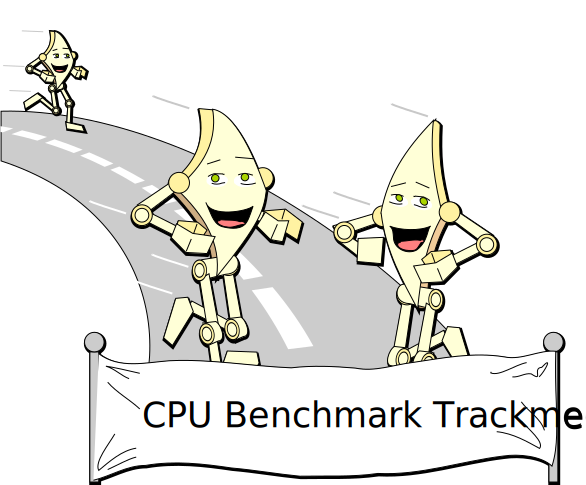
\includegraphics{cartoons/r-2014-CPU-track-meet}}
\caption{CPU Performance at its Best}
\ContributedBy{Figure}{fig:cpu:CPU Performance at its Best}{Melissa Broussard}
\end{figure}

Figure~\ref{fig:cpu:CPU Performance at its Best} 에 보여진 이상적 상황으로
접근하는 CPU 바운드 벤치마크들도 몇개 있긴 합니다만, 일반적인 프로그램은 경주용
운동장보다는 장애물 코스에 더 가깝습니다.
무어의 법칙에 의해 CPU 의 내부 구조가 지난 수십년간 엄청나게 변해왔기 때문이죠.
이런 변경들을 다음 섹션들에서 설명합니다.
\iffalse

Although there are a few CPU-bound benchmarks that approach the ideal
shown in Figure~\ref{fig:cpu:CPU Performance at its Best},
the typical program more closely resembles an obstacle course than
a race track.
This is because the internal architecture of CPUs has changed dramatically
over the past few decades, courtesy of Moore's Law.
These changes are described in the following sections.
\fi

\subsection{Pipelined CPUs}
\label{sec:cpu:Pipelined CPUs}

\begin{figure}[tb]
\centering
\resizebox{3in}{!}{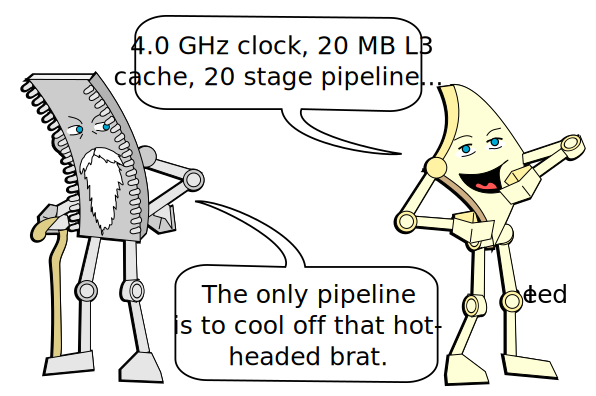
\includegraphics{cartoons/r-2014-Old-man-and-Brat}}
\caption{CPUs Old and New}
\ContributedBy{Figure}{fig:cpu:CPUs Old and New}{Melissa Broussard}
\end{figure}

1980년대 초, 인스트럭션을 가져오고, 디코드하고, 실행하는 대부분의 마이크로
프로세서는 일반적으로 다음 인스트럭션을 가져오기 전에 인스트럭션 하나를 실행
완료하는데 \emph{최소} 3 클락 사이클을 소모했습니다.
대조적으로, 1990년대 후반에서 2000년대 초반의 CPU 는 CPU 로의 인스트럭션 전달
흐름을 내부적으로 조절하는데 깊은 ``파이프라인'' 을 사용해 많은 인스트럭션들을
동시에 수행할 수 있습니다.
이러한 근래의 하드웨어의 기능들은 Figure~\ref{fig:cpu:CPUs Old and New} 에
보여진 것처럼 성능을 대폭 향상시킬 수 있습니다.
\iffalse

In the early 1980s, the typical microprocessor fetched an instruction,
decoded it, and executed it, typically taking \emph{at least} three
clock cycles to complete one instruction before proceeding to the next.
In contrast, the CPU of the late 1990s and early 2000s will be executing
many instructions simultaneously, using a deep ``pipeline'' to control
the flow of instructions internally to the CPU.
These modern hardware features can greatly improve performance, as
illustrated by Figure~\ref{fig:cpu:CPUs Old and New}.
\fi

긴 파이프라인을 가지고 CPU 의 최대 성능을 얻기 위해서는 프로그램의 컨트롤
플로우 (코드 실행 흐름) 를 매우 정밀하게 예측할 수 있어야 합니다.
큰 행렬이나 벡터 계산과 같이 기본적으로 꽉 짜여진 루프로 구성된 프로그램에서는
적당한 컨트롤 플로우를 얻을 수 있습니다.
그런 경우 CPU 는 루프 마지막의, 루프의 처음으로 돌아갈지 루프를 빠져나갈지에
대한 분기  조건이 거의 항상 참일 거라는 것을 올바르게 예측해서 파이프라인이
꽉 차있게 해 CPU가 최대 속도로 돌아갈 수 있게 할겁니다.
\iffalse

Achieving full performance with a CPU having a long pipeline requires
highly predictable control flow through the program.
Suitable control flow can be provided by a program that executes primarily
in tight loops, for example, arithmetic on large matrices or vectors.
The CPU can then correctly predict that the branch at the end of the loop
will be taken in almost all cases,
allowing the pipeline to be kept full and the CPU to execute at full speed.
\fi

\begin{figure}[tb]
\centering
\resizebox{3in}{!}{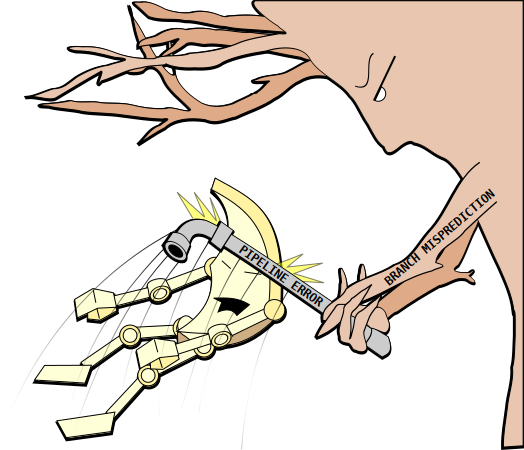
\includegraphics{cartoons/r-2014-branch-error}}
\caption{CPU Meets a Pipeline Flush}
\ContributedBy{Figure}{fig:cpu:CPU Meets a Pipeline Flush}{Melissa Broussard}
\end{figure}

하지만, 분기 예측이 항상 그렇게 쉬운건 아닙니다.
예를 들어, 작지만 무작위적인 횟수만큼 도는 많은 루프로 구성된 프로그램을
생각해보세요.
또다른 예로, 수많은 진짜 객체를 레퍼런스 할 수 있는 가상 객체들이 있는데, 이
진짜 객체들은 자주 호출되는 멤버 함수들을 모두 다르게 구현한 객체지향
프로그램을 생각해보세요.
이런 경우, CPU 는 다음 분기가 실행 흐름을 어디로 이끌지를 예측하는 건 어렵거나
심지어 불가능할 수 있습니다.
그렇게 되면 CPU 는 그 브랜치가 어디로 실행 흐름을 이끌지가 확실해질 때까지
기다리며 멈춰있거나, 추측이라도 해야 합니다.
예측 가능한 컨트롤 플로우를 갖는 프로그램에서는 추측하는 방법이 매우 잘
동작하지만, (이진 탐색과 같은) 예측 불가능한 분기분들에 대해서는 추측이 대부분
틀릴 겁니다.
추측이 잘못된 경우 CPU 는 그 분기문을 따르는, 투기적으로 그간 수행된
인스트럭션들을 모두 폐기시켜야 해서 파이프라인의 내용을 모두 비우게 되기 때문에
잘못된 예측은 매우 비싼 비용을 지불합니다.
만약 파이프라인 플러시가 너무 자주 일어난다면,
Figure~\ref{fig:cpu:CPU Meets a Pipeline Flush} 에서 그려진 것처럼 엄청난 성능
하락을 겪을 수 있습니다.
\iffalse

However, branch prediction is not always so easy.
For example, consider a program with many loops, each of which iterates
a small but random number of times.
For another example, consider
an object-oriented program with many virtual objects that
can reference many different real objects, all with different implementations
for frequently invoked member functions.
In these cases, it is difficult or even
impossible for the CPU to predict where the next branch might lead.
Then either the CPU must stall waiting for execution to proceed far
enough to be certain where that branch leads, or it must guess.
Although guessing works extremely well for programs with predictable
control flow, for unpredictable branches (such as those in binary search)
the guesses will frequently be wrong.
A wrong guess can be expensive because the CPU must discard any
speculatively executed instructions following the corresponding
branch, resulting in a pipeline flush.
If pipeline flushes appear too frequently, they drastically reduce
overall performance, as fancifully depicted in
Figure~\ref{fig:cpu:CPU Meets a Pipeline Flush}.
\fi

불행히도, 파이프라인 플러시는 근래의 CPU 들이 달려야 하는 장애물 코스의 유일한
위험이 아닙니다.
다음 섹션에서는 메모리 참조에 존재하는 위험들을 다룹니다.
\iffalse

Unfortunately, pipeline flushes are not the only hazards in the obstacle
course that modern CPUs must run.
The next section covers the hazards of referencing memory.
\fi

\subsection{Memory References}
\label{sec:cpu:Memory References}

1980년대에는, 대부분의 경우 마이크로프로세서가 메모리에서 값을 하나 얻어오는데
걸리는 시간이 인스트럭션 하나를 수행하는데 걸리는 시간보다 적었습니다.
2006년에 와서는, 마이크로프로세서는 메모리에 접근 한번 하는데 걸리는 시간 동안
수백, 심한 경우 수천개의 인스트럭션을 수행할 수 있습니다.
이 간극은 Moore 의 법칙이 CPU 성능 향상을 메모리 반응속도의 감소 정도에 비해
너무 크게 이끌었기 때문입니다; 메모리의 발전은 반응속도 감소보다 용량 증가에
치중되었던 것도 한 이유죠.
예를 들어, 1970년대의 평범한 미니컴퓨터는 4KB (네, 메가바이트가 아니라
킬로바이트요. 기가바이트는 입밖에 꺼내지도 마요) 메인 메모리를 가졌고, 그
메모리는 한 사이클만에 접근 가능했습니다.\footnote{
	물론 그 한개의 사이클은 1.6 \emph{마이크로 세컨드} 이상이었음을
	언급하는게 공정하겠죠.}
2008년에도 CPU 설계자들은 여전히 단일 사이클만에 접근 가능한 4KB 메모리를 만들
수 있습니다; 심지어 수 GHz 주파수의 시스템에서도요.
그리고 실제로 그런 메모리를 만듭니다만, 그들은 이제 그걸 ``레벨 0 캐시'' 라
부르고, 그것들은 보통은 4KB 보다는 아주 약간은 크기도 합니다.
\iffalse

In the 1980s, it often took less time for a microprocessor to load a value
from memory than it did to execute an instruction.
In 2006, a microprocessor might be capable of executing hundreds or even
thousands of instructions in the time required to access memory.
This disparity is due to the fact that Moore's Law has increased CPU
performance at a much greater rate than it has decreased memory latency,
in part due to the rate at which memory sizes have grown.
For example, a typical 1970s minicomputer might have 4\,KB (yes, kilobytes,
not megabytes, let alone gigabytes) of main memory, with
single-cycle access.\footnote{
	It is only fair to add that each of these single cycles
	lasted no less than 1.6 \emph{microseconds}.}
In 2008, CPU designers still can construct a 4\,KB memory with single-cycle
access, even on systems with multi-GHz clock frequencies.
And in fact they frequently do construct such memories, but they now
call them ``level-0 caches'', and they can be quite a bit bigger than 4\,KB.
\fi

\begin{figure}[htb]
\centering
\resizebox{3in}{!}{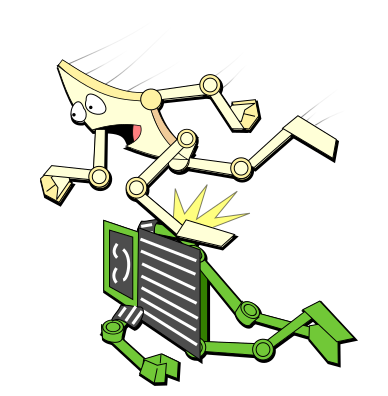
\includegraphics{cartoons/r-2014-memory-reference}}
\caption{CPU Meets a Memory Reference}
\ContributedBy{Figure}{fig:cpu:CPU Meets a Memory Reference}{Melissa Broussard}
\end{figure}

근래의 마이크로프로세서에 장착되는 큰 캐시들은 메모리 접근 시간과 맞서 싸우는데
꽤 도움을 줄 수 있습니다만, 이런 캐시들이 그 시간들을 제대로 숨기기 위해서는
고도로 예측 가능한 데이터 접근 패턴이 필요합니다.
불행히도, 링크드 리스트를 순회하는 것과 같은 많은 일들이 예측 불가능한 메모리
접근 패턴을 갖습니다. 무엇보다, 만약 패턴이 예측 가능하다면, 소프트웨어는
포인터 타입이란 것 자체를 만들지도 않았겠죠, 그렇죠?
따라서, Figure~\ref{fig:cpu:CPU Meets a Memory Reference} 에서 보여지듯, 메모리
참조는 종종 근래의 CPU 들에게 거대한 장애물입니다.

지금까지는 주어진 CPU가 싱글 쓰레드 코드를 돌릴 때 만날 수 있는 문제들만
이야기했습니다.
멀티쓰레드 수행은 다음 섹션에서 설명할텐데, CPU 에게 추가적인 문제들을
내놓습니다.
\iffalse

Although the large caches found on modern microprocessors can do quite
a bit to help combat memory-access latencies,
these caches require highly predictable data-access patterns to
successfully hide those latencies.
Unfortunately, common operations such as traversing a linked list
have extremely unpredictable memory-access patterns---after all,
if the pattern was predictable, us software types would not bother
with the pointers, right?
Therefore, as shown in
Figure~\ref{fig:cpu:CPU Meets a Memory Reference},
memory references often pose severe obstacles to modern CPUs.

Thus far, we have only been considering obstacles that can arise during
a given CPU's execution of single-threaded code.
Multi-threading presents additional obstacles to the CPU, as
described in the following sections.
\fi

\subsection{Atomic Operations}
\label{sec:cpu:Atomic Operations}

그런 장애 중 하나는 어토믹 오퍼레이션들입니다.
여기서의 문제는 모든 어토믹 오퍼레이션은 CPU 파이프라인의 한 순간에는 조각으로
나뉘어 수행되는 어셈블리 오퍼레이션들과 한번씩은 충돌한다는 것입니다.
하드웨어 설계자는 근래의 CPU 들은 그런 오퍼레이션들이 실은 여러 조각으로
나뉘어져 여러 순간동안 수행되더라도 원자적으로 수행되는 것처럼 \emph{보이게}
하기 위해 여러개의 굉장히 현명한 트릭들을 사용한다고 이야기합니다. 그런 트릭 중
흔한 한가지는 어토믹하게 수행되어야 하는 데이터를 담고 있는 캐시라인들을 모두
파악해두고, 이 캐시라인들은 해당 어토믹 오퍼레이션을 수행하는 CPU 에 소유되어
있음을 분명하게 하고, 그러고나서야만 해당 캐시라인들이 해당 CPU 에 의해 여전히
소유되어 있음을 분명히 한 채로 어토믹 오퍼레이션을 수행하는 것입니다.
모든 데이터가 해당 CPU 만 접근할 수 있는 상태이기에, 다른 CPU 들은 실은
조각으로 나뉘어 수행되는 CPU 파이프라인의 현실에도 불구하고 해당 어토믹
오퍼레이션에 간섭을 끼칠 수 없습니다.
말할 필요도 없겠지만, 이런 종류의 트릭은 그 셋업이 수행되도록 주어진 어토믹
오퍼레이션이 완전히 끝날 때까지 파이프라인이 지연되거나 심지어 플러시될 수도
있습니다.

\iffalse
One such obstacle is atomic operations.
The problem here is that the whole idea of an atomic operation conflicts with
the piece-at-a-time assembly-line operation of a CPU pipeline.
To hardware designers' credit, modern CPUs use a number of extremely clever
tricks to make such operations \emph{look} atomic even though they
are in fact being executed piece-at-a-time,
with one common trick being to identify all the cachelines containing the
data to be atomically operated on,
ensure that these cachelines are owned by the CPU executing the
atomic operation, and only then proceed with the atomic operation
while ensuring that these cachelines remained owned by this CPU.
Because all the data is private to this CPU, other CPUs are unable to
interfere with the atomic operation despite the piece-at-a-time nature
of the CPU's pipeline.
Needless to say, this sort of trick can require that
the pipeline must be delayed or even flushed in order to
perform the setup operations that
permit a given atomic operation to complete correctly.
\fi

\begin{figure}[htb]
\centering
\resizebox{3in}{!}{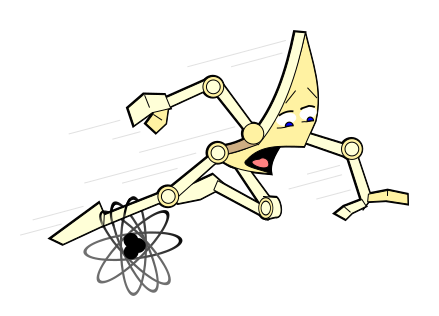
\includegraphics{cartoons/r-2014-Atomic-reference}}
\caption{CPU Meets an Atomic Operation}
\ContributedBy{Figure}{fig:cpu:CPU Meets an Atomic Operation}{Melissa Broussard}
\end{figure}

반대로, 어토믹 오퍼레이션이 아닌 오퍼레이션을 수행할 때에는 CPU 는 값을
캐시라인에 올라오는대로 가져올 수 있고, 수행 결과를 캐시라인 소유권을 가지기
위해 기다릴 필요 없이 곧바로 버퍼에 써넣을 수 있습니다.
다행히도, CPU 설계자들은 어토믹 오퍼레이션에 신경을 많이 쏟았고, 덕분에 2014년
초에 이르러서는 그 오버헤드를 상당히 감소시켰습니다.
하지만 그래도, 그 성능에 끼치는 효과는 Figure~\ref{fig:cpu:CPU Meets an Atomic
Operation} 에 보이는 대로입니다.

불행히도, 어토믹 오퍼레이션들은 보통 데이터의 한개 요소에만 적용 가능합니다.
많은 병렬 알고리즘들이 복수개의 데이터 요소들에의 업데이트 간에도 순서가
이루어지길 필요로 하기 때문에, 대부분의 CPU 들은 메모리 배리어들을 제공합니다.
이런 메모리 배리어들 역시 성능에의 문제로 존재합니다. 다음 섹션에서 이를 이야기
합니다.

\iffalse
In contrast, when executing a non-atomic operation, the CPU can load
values from cachelines as they appear and place the results in the
store buffer, without the need to wait for cacheline ownership.
Fortunately, CPU designers have focused heavily on atomic operations,
so that as of early 2014 they have greatly reduced their overhead.
Even so, the resulting effect on performance is all too often as depicted in
Figure~\ref{fig:cpu:CPU Meets an Atomic Operation}.

Unfortunately, atomic operations usually apply only to single elements
of data.
Because many parallel algorithms require that ordering constraints
be maintained between updates of multiple data elements, most CPUs
provide memory barriers.
These memory barriers also serve as performance-sapping obstacles,
as described in the next section.
\fi

\QuickQuiz{}
	어떤 기계가 복수 데이터 요소에 대한 어토믹 오퍼레이션을 허용하겠어요?

	\iffalse
	What types of machines would allow atomic operations on
	multiple data elements?
	\fi
\QuickQuizAnswer{
	이 질문에 대한 한가지 답은 종종 복수개의 데이터 요소를 어토믹하게
	다뤄질 수 있는, 단일 머신 워드 안에 모아넣을 수 있다는 겁니다.

	좀 더 트렌디한 답은 트랜잭셔널 메모리~\cite{DBLomet1977SIGSOFT} 를
	지원하는 기계가 되겠습니다.
	2014년 초에 이르러서는 일부 주요 시스템들이 제한되긴 했지만 하드웨어
	트랜잭셔널 메모리 구현을 제공합니다. 더 자세한 내용은
	Section~\ref{sec:future:Hardware Transactional Memory} 에서 다루고
	있습니다.
	소프트웨어 트랜잭셔널
	메모리~\cite{McKenney2007PLOSTM,DonaldEPorter2007TRANSACT,
	ChistopherJRossbach2007a,CalinCascaval2008tmtoy,
	AleksandarDragovejic2011STMnotToy,AlexanderMatveev2012PessimisticTM}
	에 대해서는 아직 적합하지 않다는 평가입니다.
	소프트웨어 트랜잭셔널 메모리에 대한 더 많은 내용은
	Section~\ref{sec:future:Transactional Memory} 에서 볼 수 있을 겁니다.

	\iffalse
	One answer to this question is that it is often possible to
	pack multiple elements of data into a single machine word,
	which can then be manipulated atomically.

	A more trendy answer would be machines supporting transactional
	memory~\cite{DBLomet1977SIGSOFT}.
	As of early 2014, several mainstream systems provide limited
	hardware transactional memory implementations, which is covered
	in more detail in
	Section~\ref{sec:future:Hardware Transactional Memory}.
	The jury is still out on the applicability of software transactional
	memory~\cite{McKenney2007PLOSTM,DonaldEPorter2007TRANSACT,
	ChistopherJRossbach2007a,CalinCascaval2008tmtoy,
	AleksandarDragovejic2011STMnotToy,AlexanderMatveev2012PessimisticTM}.
	Additional information on software transactional memory may be
	found in
	Section~\ref{sec:future:Transactional Memory}.
	\fi
} \QuickQuizEnd

\subsection{Memory Barriers}
\label{sec:cpu:Memory Barriers}

메모리 배리어에 대해서는
Chapter~\ref{chp:Advanced Synchronization: Memory Ordering} 와
Appendix~\ref{chp:app:whymb:Why Memory Barriers?} 에서 좀 더 깊게 다룰 겁니다.
그 전에, 여기서는 다음의 간단한 락을 사용한 크리티컬 섹션을 생각해 봅시다:

\iffalse
Memory barriers will be considered in more detail in
Chapter~\ref{chp:Advanced Synchronization: Memory Ordering} and
Appendix~\ref{chp:app:whymb:Why Memory Barriers?}.
In the meantime, consider the following simple lock-based critical
section:
\fi

\vspace{5pt}
\begin{minipage}[t]{\columnwidth}
\small
\begin{verbatim}
  1 spin_lock(&mylock);
  2 a = a + 1;
  3 spin_unlock(&mylock);
\end{verbatim}
\end{minipage}
\vspace{5pt}

\begin{figure}[tb]
\centering
\resizebox{3in}{!}{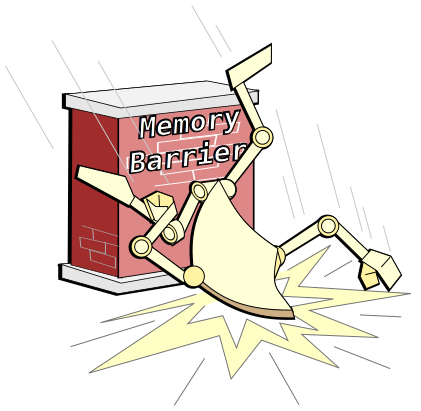
\includegraphics{cartoons/r-2014-Memory-barrier}}
\caption{CPU Meets a Memory Barrier}
\ContributedBy{Figure}{fig:cpu:CPU Meets a Memory Barrier}{Melissa Broussard}
\end{figure}

만약 CPU 에 코드가 보여지는 순서대로 수행되어야 한다는 제약이 존재하지
않는다면, 변수 ``a'' 는 ``mylock'' 의 보호 없이 값이 증가할 것이고, 이렇게 되면
락을 잡는 목표가 이뤄지지 않은 셈입니다.
그런 문제되는 순서 재배치를 막기 위해, 락킹에 사용되는 기본 기능들은 명시적이든
묵시적이든 메모리 배리어를 사용합니다.
이런 메모리 배리어의 목적은 CPU 가 성능을 향상시키기 위해 할 수 있는 코드의
순서 재배치를 막기 위한 것이기 때문에, 메모리 배리어는 거의 항상
Figure~\ref{fig:cpu:CPU Meets a Memory Barrier} 에서 보여지듯 성능을
떨어뜨립니다.

어토믹 오퍼레이션과 같이, CPU 설계자들은 메모리 배리어 오버헤드를 줄이려 열심히
노력해왔고, 꽤 많은 진전을 이뤘습니다.

\iffalse
If the CPU were not constrained to execute these statements in the
order shown, the effect would be that the variable ``a'' would be
incremented without the protection of ``mylock'', which would certainly
defeat the purpose of acquiring it.
To prevent such destructive reordering, locking primitives contain
either explicit or implicit memory barriers.
Because the whole purpose of these memory barriers is to prevent reorderings
that the CPU would otherwise undertake in order to increase performance,
memory barriers almost always reduce performance, as depicted in
Figure~\ref{fig:cpu:CPU Meets a Memory Barrier}.

As with atomic operations, CPU designers have been working hard to
reduce memory-barrier overhead, and have made substantial progress.
\fi

\subsection{Cache Misses}
\label{sec:cpu:Cache Misses}

\begin{figure}[tb]
\centering
\resizebox{3in}{!}{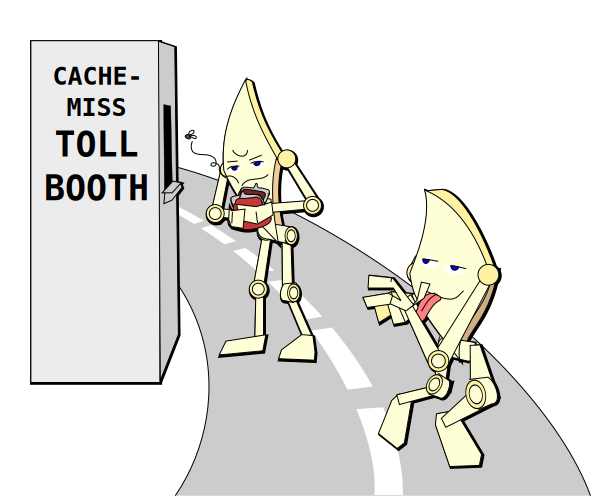
\includegraphics{cartoons/r-2014-CPU-track-meet-cache-miss-toll-booth}}
\caption{CPU Meets a Cache Miss}
\ContributedBy{Figure}{fig:cpu:CPU Meets a Cache Miss}{Melissa Broussard}
\end{figure}

또하나의 멀티 쓰레딩에서의 CPU 성능에의 장애물은 ``캐시 미스'' 입니다.
앞서 말했듯, 근래의 CPU 들은 높은 메모리 반응속도로 발생할 수 있는 성능 하락을
줄이기 위해 큰 캐시를 장착하고 있습니다.
하지만, 이런 캐시들은 실은 CPU 간에 자주 공유되는 변수들에 대해서는 생산적이지
못합니다.
하나의 CPU 가 한 변수를 수정하려 할 때, 다른 CPU 가 그 값을 최근에 바꾼 경우가
있을 가능성이 크기 때문이죠.
이런 경우, 해당 변수는 지금 수정하려는 CPU 의 캐시가 아니라 최근에 값을 수정한
CPU 의 캐시에 있을 것이고, 이로 인해 비싼 캐시 미스(더 자세한 내용을 위해선
Section~\ref{sec:app:whymb:Cache Structure} 를 보세요) 를 일으킬 것입니다.
이런 캐시 미스들은 Figure~\ref{fig:cpu:CPU Meets a Cache Miss} 에서 보여진
것처럼 CPU 성능의 주요 장애가 됩니다.

\iffalse
An additional multi-threading obstacle to CPU performance is
the ``cache miss''.
As noted earlier, modern CPUs sport large caches in order to reduce the
performance penalty that would otherwise be incurred due to high memory
latencies.
However, these caches are actually counter-productive for variables that
are frequently shared among CPUs.
This is because when a given CPU wishes to modify the variable, it is
most likely the case that some other CPU has modified it recently.
In this case, the variable will be in that other CPU's cache, but not
in this CPU's cache, which will therefore incur an expensive cache miss
(see Section~\ref{sec:app:whymb:Cache Structure} for more detail).
Such cache misses form a major obstacle to CPU performance, as shown
in Figure~\ref{fig:cpu:CPU Meets a Cache Miss}.
\fi

\QuickQuiz{}
	그래서, CPU 설계자들은 캐시 미스 오버헤드 역시 많이 개선 했나요?
	\iffalse
	So have CPU designers also greatly reduced the overhead of
	cache misses?
	\fi
\QuickQuizAnswer{
	안타깝지만, 그렇게 많은 개선은 하지 못했습니다.
	약간 오버헤드를 줄인 CPU 들도 있었습니다만, 빛의 속도의 한계와 물질의
	원자성의 자연 법칙이 큰 시스템에서 캐시 미스 오버헤드를 줄일 수 있는
	방법을 제한하고 있습니다.
	Section~\ref{sec:cpu:Hardware Free Lunch?} 에서 가능할 법한 미래의 개선
	방법들을 논의해 봅니다.

	\iffalse
	Unfortunately, not so much.
	There has been some reduction given constant numbers of CPUs,
	but the finite speed of light and the atomic nature of
	matter limits their ability to reduce cache-miss overhead
	for larger systems.
	Section~\ref{sec:cpu:Hardware Free Lunch?}
	discusses some possible avenues for possible future progress.
	\fi
} \QuickQuizEnd

\subsection{I/O Operations}
\label{sec:cpu:I/O Operations}

\begin{figure}[tb]
\centering
\resizebox{3in}{!}{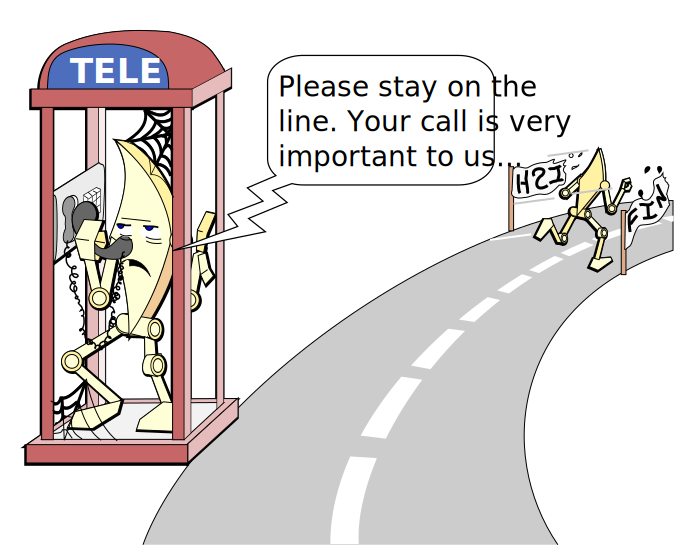
\includegraphics{cartoons/r-2014-CPU-track-meet-phone-booth}}
\caption{CPU Waits for I/O Completion}
\ContributedBy{Figure}{fig:cpu:CPU Waits for I/O Completion}{Melissa Broussard}
\end{figure}

캐시 미스는 곧 CPU 와 CPU 사이의 I/O 오퍼레이션으로 볼 수 있고, 이것은 가능한
I/O 오퍼레이션 중 가장 비용이 낮은 것들 중 하나입니다.
네트워킹이나 대용량 저장장치, 또는 사람을 포함하는 I/O 오퍼레이션들은
Figure~\ref{fig:cpu:CPU Waits for I/O Completion} 에서 보여지듯, 앞의
섹션들에서 이야기 되었던 내부적 장애들보다 훨씬 커다란 장애를 야기합니다.

\iffalse
A cache miss can be thought of as a CPU-to-CPU I/O operation, and as
such is one of the cheapest I/O operations available.
I/O operations involving networking, mass storage, or (worse yet) human
beings pose much greater obstacles than the internal obstacles called
out in the prior sections,
as illustrated by
Figure~\ref{fig:cpu:CPU Waits for I/O Completion}.
\fi

이건 공유 메모리 병렬성과 분산시스템 병렬성 사이의 차이 중 하나입니다:
공유메모리 병렬 프로그램은 일반적으로 캐시 미스보다 더한 장애는 겪지
않습니다만, 분산 병렬 프로그램은 보통 더 큰 네트워크 커뮤니케이션 시간을
겪습니다.
두 경우 모두, 문제의 응답시간들은 커뮤니케이션의 비용으로 생각될 수 있습니다.
순차 프로그램에서는 존재하지 않는 비용이죠.
따라서, 실제 수행되는 일과 커뮤니케이션 오버헤드 간의 비율이 핵심 설계 결정
요소입니다.
병렬 하드웨어 설계의 주요 목표는 이 비율을 적절한 성능과 확장성 목표를 달성
가능한 수준으로 낮추는 것입니다.
이에 따라서, Chapter~\ref{cha:Partitioning and Synchronization Design} 에서
볼테지만, 병렬 소프트웨어 설계의 중요한 목표는 커뮤니케이션 캐시 미스와 같은
비싼 동작들의 빈번도를 낮추는 것입니다.

물론, 주어진 동작이 장애라는 이야기는 그 이야기이고, 그 동작이 \emph{심각한}
장애라는 건 또 따로 보여줘야하지요.
이 차이를 다음의 섹션에서 이야기 합니다.

\iffalse
This is one of the differences between shared-memory and distributed-system
parallelism: shared-memory parallel programs must normally deal with no
obstacle worse than a cache miss, while a distributed parallel program
will typically incur the larger network communication latencies.
In both cases, the relevant latencies can be thought of as a cost of
communication---a cost that would be absent in a sequential program.
Therefore, the ratio between the overhead of the communication to
that of the actual work being performed is a key design parameter.
A major goal of parallel hardware design is to reduce this ratio as
needed to achieve the relevant performance and scalability goals.
In turn, as will be seen in
Chapter~\ref{cha:Partitioning and Synchronization Design},
a major goal of parallel software design is to reduce the
frequency of expensive operations like communications cache misses.

Of course, it is one thing to say that a given operation is an obstacle,
and quite another to show that the operation is a \emph{significant}
obstacle.
This distinction is discussed in the following sections.
\fi

% cpu/overheads.tex
% mainfile: ../perfbook.tex
% SPDX-License-Identifier: CC-BY-SA-3.0

\section{Overheads}
\label{sec:cpu:Overheads}
%
\epigraph{Don't design bridges in ignorance of materials, and don't design
	  low-level software in ignorance of the underlying hardware.}
	 {\emph{Unknown}}

This section presents actual overheads of the obstacles to performance
listed out in the previous section.
However, it is first necessary to get a rough view of hardware system
architecture, which is the subject of the next section.

\subsection{Hardware System Architecture}
\label{sec:cpu:Hardware System Architecture}

\begin{figure}[tb]
\centering
\resizebox{3in}{!}{\includegraphics{cpu/SystemArch}}
\caption{System Hardware Architecture}
\label{fig:cpu:System Hardware Architecture}
\end{figure}

Figure~\ref{fig:cpu:System Hardware Architecture}
shows a rough schematic of an eight-core computer system.
Each die has a pair of CPU cores, each with its cache, as well as an
interconnect allowing the pair of CPUs to communicate with each other.
The system interconnect allows the four dies to communicate with each
other and with main memory.

Data moves through this system in units of ``cache lines'', which
are power-of-two fixed-size aligned blocks of memory, usually ranging
from 32 to 256 bytes in size.
When a CPU loads a variable from memory to one of its registers, it must
first load the cacheline containing that variable into its cache.
Similarly, when a CPU stores a value from one of its registers into
memory, it must also load the cacheline containing that variable into
its cache, but must also ensure that no other CPU has a copy of that
cacheline.

For example, if CPU~0 were to write to a variable whose cacheline
resided in CPU~7's cache, the following over-simplified sequence of
events might ensue:

\begin{enumerate}
\item	CPU~0 checks its local cache, and does not find the cacheline.
	It therefore records the write in its store buffer.
\item	A request for this cacheline is forwarded to CPU~0's and 1's
	interconnect, which checks CPU~1's local cache, and does not
	find the cacheline.
\item	This request is forwarded to the system interconnect, which
	checks with the other three dies, learning that the cacheline
	is held by the die containing CPU~6 and 7.
\item	This request is forwarded to CPU~6's and 7's interconnect, which
	checks both CPUs' caches, finding the value in CPU~7's cache.
\item	CPU~7 forwards the cacheline to its interconnect, and also
	flushes the cacheline from its cache.
\item	CPU~6's and 7's interconnect forwards the cacheline to the
	system interconnect.
\item	The system interconnect forwards the cacheline to CPU~0's and 1's
	interconnect.
\item	CPU~0's and 1's interconnect forwards the cacheline to CPU~0's
	cache.
\item	CPU~0 can now complete the write, updating the relevant portions
	of the newly arrived cacheline from the value previously
	recorded in the store buffer.
\end{enumerate}

\QuickQuizSeries{%
\QuickQuizB{
	This is a \emph{simplified} sequence of events?
	How could it \emph{possibly} be any more complex?
}\QuickQuizAnswerB{
	This sequence ignored a number of possible complications,
	including:

	\begin{enumerate}
	\item	Other CPUs might be concurrently attempting to perform
		memory-reference operations involving this same cacheline.
	\item	The cacheline might have been replicated read-only in
		several CPUs' caches, in which case, it would need to
		be flushed from their caches.
	\item	CPU~7 might have been operating on the cache line when
		the request for it arrived, in which case CPU~7 might
		need to hold off the request until its own operation
		completed.
	\item	CPU~7 might have ejected the cacheline from its cache
		(for example, in order to make room for other data),
		so that by the time that the request arrived, the
		cacheline was on its way to memory.
	\item	A correctable error might have occurred in the cacheline,
		which would then need to be corrected at some point before
		the data was used.
	\end{enumerate}

	Production-quality cache-coherence mechanisms are extremely
	complicated due to these sorts of
	considerations~\cite{Hennessy95a,DavidECuller1999,MiloMKMartin2012scale,DanielJSorin2011MemModel}.
%
}\QuickQuizEndB
%
\QuickQuizE{
	Why is it necessary to flush the cacheline from CPU~7's cache?
}\QuickQuizAnswerE{
	If the cacheline was not flushed from CPU~7's cache, then
	CPUs~0 and 7 might have different values for the same set
	of variables in the cacheline.
	This sort of incoherence greatly complicates parallel software,
	which is why so wise hardware architects avoid it.
}\QuickQuizEndE
}

This simplified sequence is just the beginning of a discipline called
\emph{cache-coherency protocols}~\cite{Hennessy95a,DavidECuller1999,MiloMKMartin2012scale,DanielJSorin2011MemModel},
which is discussed in more detail in
Appendix~\ref{chp:app:whymb:Why Memory Barriers?}.
As can be seen in the sequence of events triggered by a CAS operation,
a single instruction can cause considerable protocol traffic, which
can significantly degrade your parallel program's performance.

Fortunately, if a given variable is being frequently read during a time
interval during which it is never updated, that variable can be replicated
across all CPUs' caches.
This replication permits all CPUs to enjoy extremely fast access to
this \emph{read-mostly} variable.
Chapter~\ref{chp:Deferred Processing} presents synchronization
mechanisms that take full advantage of this important hardware read-mostly
optimization.

\subsection{Costs of Operations}
\label{sec:cpu:Costs of Operations}

\begin{table*}
\rowcolors{1}{}{lightgray}
\renewcommand*{\arraystretch}{1.1}
\centering\small
\begin{tabular}
  {
    l
    S[table-format = 9.1]
    S[table-format = 9.1]
    r
  }
	\toprule
	Operation	   & \multicolumn{1}{r}{Cost (ns)}
				   & {\parbox[b]{.7in}{\raggedleft Ratio\\(cost/clock)}}
					    & CPUs \\
	\midrule
	Clock period		     &   0.5 &    1.0 &			  \\
	Same-CPU CAS		     &   7.0 &   14.6 & 0		  \\
	Same-CPU lock		     &  15.4 &   32.3 & 0		  \\
	In-core blind CAS	     &   7.2 &   15.2 & 224		  \\
	In-core CAS		     &  18.0 &   37.7 & 224		  \\
	Off-core blind CAS	     &  47.5 &   99.8 & 1--27,225--251	  \\
	Off-core CAS		     & 101.9 &  214.0 & 1--27,225--251	  \\
	Off-socket blind CAS	     & 148.8 &  312.5 & 28--111,252--335  \\
	Off-socket CAS		     & 442.9 &  930.1 & 28--111,252--335  \\
	Cross-interconnect blind CAS & 336.6 &  706.8 & 112--223,336--447 \\
	Cross-interconnect CAS	     & 944.8 & 1984.2 & 112--223,336--447 \\
	\midrule
	Off-System	&	      & 	    & \\
	Comms Fabric	&       5 000 &      10 500 & \\
	Global Comms	& 195 000 000 & 409 500 000 & \\
	\bottomrule
\end{tabular}
\caption{CPU 0 View of Synchronization Mechanisms on 8-Socket System With Intel Xeon Platinum 8176 CPUs @ 2.10\,GHz}
\label{tab:cpu:CPU 0 View of Synchronization Mechanisms on 8-Socket System With Intel Xeon Platinum 8176 CPUs at 2.10GHz}
\end{table*}

The overheads of some common operations important to parallel programs are
displayed in
Table~\ref{tab:cpu:CPU 0 View of Synchronization Mechanisms on 8-Socket System With Intel Xeon Platinum 8176 CPUs at 2.10GHz}.
This system's clock period rounds to 0.5\,ns.
Although it is not unusual for modern microprocessors to be able to
retire multiple instructions per clock period, the operations' costs are
nevertheless normalized to a clock period in the third column, labeled
``Ratio''.
The first thing to note about this table is the large values of many of
the ratios.

The same-CPU compare-and-swap (CAS) operation consumes about seven
nanoseconds, a duration more than ten times that of the clock period.
CAS is an atomic operation in which the hardware compares the contents
of the specified memory location to a specified ``old'' value, and if
they compare equal, stores a specified ``new'' value, in which case the
CAS operation succeeds.
If they compare unequal, the memory location keeps its (unexpected) value,
and the CAS operation fails.
The operation is atomic in that the hardware guarantees that the memory
location will not be changed between the compare and the store.
CAS functionality is provided by the \co{lock;cmpxchg} instruction on x86.

The ``same-CPU'' prefix means that the CPU now performing the CAS operation
on a given variable was also the last CPU to access this variable, so
that the corresponding cacheline is already held in that CPU's cache.
Similarly, the same-CPU lock operation (a ``round trip'' pair consisting
of a lock acquisition and release) consumes more than fifteen nanoseconds,
or more than thirty clock cycles.
The lock operation is more expensive than CAS because it requires two
atomic operations on the lock data structure, one for acquisition and
the other for release.

In-core operations involving interactions between the hardware threads
sharing a single core are about the same cost as same-CPU operations.
This should not be too surprising, given that these two hardware threads
also share the full cache hierarchy.

In the case of the blind CAS, the software specifies the old value
without looking at the memory location.
This approach is appropriate when attempting to acquire a lock.
If the unlocked state is represented by zero and the locked state
is represented by the value one, then a CAS operation on the lock
that specifies zero for the old value and one for the new value
will acquire the lock if it is not already held.
The key point is that there is only one access to the memory
location, namely the CAS operation itself.

In contrast, a normal CAS operation's old value is derived from
some earlier load.
For example, to implement an atomic increment, the current value of
that location is loaded and that value is incremented to produce the
new value.
Then in the CAS operation, the value actually loaded would be specified
as the old value and the incremented value as the new value.
If the value had not been changed between the load and the CAS, this
would increment the memory location.
However, if the value had in fact changed, then the old value would
not match, causing a miscompare that would result in the CAS operation
failing.
The key point is that there are now two accesses to the memory location,
the load and the CAS\@.

Thus, it is not surprising that in-core blind CAS consumes only about
seven nanoseconds, while in-core CAS consumes about 18 nanoseconds.
The non-blind case's extra load does not come for free.
That said, the overhead of these operations are similar to single-CPU
CAS and lock, respectively.

\QuickQuiz{
	\Cref{tab:cpu:CPU 0 View of Synchronization Mechanisms on 8-Socket System With Intel Xeon Platinum 8176 CPUs at 2.10GHz}
	shows CPU~0 sharing a core with CPU~224.
	Shouldn't that instead be CPU~1???
}\QuickQuizAnswer{
	It is easy to be sympathetic to this view, but the file
	\path{/sys/devices/system/cpu/cpu0/cache/index0/shared_cpu_list}
	really does contain the string \co{0,224}.
	Therefore, CPU~0's hyperthread twin really is CPU~224.
	Some people speculate that this numbering allows naive applications
	and schedulers to perform better, citing the fact that on many
	workloads the second hyperthread does not provide a huge
	amount of additional performance.
	This speculation assumes that naive applications and schedulers
	would utilize CPUs in numerical order, leaving aside the weaker
	hyperthread twin CPUs until all cores are in use.
}\QuickQuizEnd

A blind CAS involving CPUs in different cores but on the same socket
consumes almost fifty nanoseconds, or almost one hundred clock cycles.
The code used for this cache-miss measurement passes the cache line
back and forth between a pair of CPUs, so this cache miss is satisfied
not from memory, but rather from the other CPU's cache.
A non-blind CAS operation, which as noted earlier must look at the old
value of the variable as well as store a new value, consumes over one
hundred nanoseconds, or more than two hundred clock cycles.
Think about this a bit.
In the time required to do \emph{one} CAS operation, the CPU could have
executed more than \emph{two hundred} normal instructions.
This should demonstrate the limitations not only of fine-grained locking,
but of any other synchronization mechanism relying on fine-grained
global agreement.

If the pair of CPUs are on different sockets, the operations are considerably
more expensive.
A blind CAS operation consumes almost 150~nanoseconds, or more than
three hundred clock cycles.
A normal CAS operation consumes more than 400~nanoseconds, or almost
\emph{one thousand} clock cycles.

Worse yet, not all pairs of sockets are created equal.
This particular system appears to be constructed as a pair of four-socket
components, with additional latency penalties when the CPUs reside
in different components.
In this case, a blind CAS operation consumes more than three hundred
nanoseconds, or more than seven hundred clock cycles.
A CAS operation consumes almost a full microsecond, or almost two
thousand clock cycles.

\QuickQuiz{
	Surely the hardware designers could be persuaded to improve
	this situation!
	Why have they been content with such abysmal performance
	for these single-instruction operations?
}\QuickQuizAnswer{
	The hardware designers \emph{have} been working on this
	problem, and have consulted with no less a luminary than
	the late physicist Stephen Hawking.
	Hawking's observation was that the hardware designers have
	two basic problems~\cite{BryanGardiner2007}:

	\begin{enumerate}
	\item	The finite speed of light, and
	\item	The atomic nature of matter.
	\end{enumerate}

\begin{table}
\rowcolors{1}{}{lightgray}
\renewcommand*{\arraystretch}{1.1}
\centering\small
\begin{tabular}
  {
    l
    S[table-format = 9.1]
    S[table-format = 9.1]
  }
	\toprule
	Operation		& \multicolumn{1}{r}{Cost (ns)}
			& {\parbox[b]{.7in}{\raggedleft Ratio\\(cost/clock)}} \\
	\midrule
	Clock period		&           0.4	&           1.0 \\
	Same-CPU CAS		&          12.2	&          33.8 \\
	Same-CPU lock		&          25.6	&          71.2 \\
	Blind CAS		&          12.9	&          35.8 \\
	CAS			&           7.0	&          19.4 \\
	\midrule
	Off-Core		&		&		\\
	Blind CAS		&          31.2	&          86.6 \\
	CAS			&          31.2	&          86.5 \\
	\midrule
	Off-Socket		&		&		\\
	Blind CAS		&          92.4	&         256.7 \\
	CAS			&          95.9	&         266.4 \\
	\midrule
	Off-System		&		&		\\
	Comms Fabric		&       2 600   &       7 220   \\
	Global Comms		& 195 000 000	& 542 000 000   \\
	\bottomrule
\end{tabular}
\caption{Performance of Synchronization Mechanisms on 16-CPU 2.8\,GHz Intel X5550 (Nehalem) System}
\label{tab:cpu:Performance of Synchronization Mechanisms on 16-CPU 2.8GHz Intel X5550 (Nehalem) System}
\end{table}

	The first problem limits raw speed, and the second limits
	miniaturization, which in turn limits frequency.
	And even this sidesteps the power-consumption issue that
	is currently limiting production frequencies to well below
	10\,GHz.

	In addition,
	Table~\ref{tab:cpu:CPU 0 View of Synchronization Mechanisms on 8-Socket System With Intel Xeon Platinum 8176 CPUs at 2.10GHz}
	on
	page~\pageref{tab:cpu:CPU 0 View of Synchronization Mechanisms on 8-Socket System With Intel Xeon Platinum 8176 CPUs at 2.10GHz}
	represents a reasonably large system with no fewer 448~hardware
	threads.
	Smaller systems often achieve better latency, as may be seen in
	Table~\ref{tab:cpu:Performance of Synchronization Mechanisms on 16-CPU 2.8GHz Intel X5550 (Nehalem) System},
	which represents a much smaller system with only 16 hardware threads.
	A similar view is provided by the rows of
	Table~\ref{tab:cpu:CPU 0 View of Synchronization Mechanisms on 8-Socket System With Intel Xeon Platinum 8176 CPUs at 2.10GHz}
	down to and including the two ``Off-core'' rows.

\begin{table*}
\rowcolors{1}{}{lightgray}
\renewcommand*{\arraystretch}{1.1}
\centering\small
\begin{tabular}
  {
    l
    S[table-format = 9.1]
    S[table-format = 9.1]
    r
  }
	\toprule
	Operation		& \multicolumn{1}{r}{Cost (ns)}
			& {\parbox[b]{.7in}{\raggedleft Ratio\\(cost/clock)}}
			& CPUs \\
	\midrule
	Clock period		     &   0.5 &    1.0 &			  \\
	Same-CPU CAS		     &   6.2 &   13.6 & 0		  \\
	Same-CPU lock		     &  13.5 &   29.6 & 0		  \\
	In-core blind CAS	     &   6.5 &   14.3 & 6		  \\
	In-core CAS		     &  16.2 &   35.6 & 6		  \\
	Off-core blind CAS	     &  22.2 &   48.8 & 1--5,7--11	  \\
	Off-core CAS		     &  53.6 &  117.9 & 1--5,7--11	  \\
	\midrule
	Off-System	&	      & 	    & \\
	Comms Fabric	&       5 000 &      11 000 & \\
	Global Comms	& 195 000 000 & 429 000 000 & \\
	\bottomrule
\end{tabular}
\caption{CPU 0 View of Synchronization Mechanisms on 12-CPU Intel Core i7-8750H CPU @ 2.20\,GHz}
\label{tab:cpu:CPU 0 View of Synchronization Mechanisms on 12-CPU Intel Core i7-8750H CPU @ 2.20GHz}
\end{table*}

	Furthermore, newer small-scale single-socket systems such
	as the laptop on which I am typing this also have more
	reasonable latencies, as can be seen in
	\cref{tab:cpu:CPU 0 View of Synchronization Mechanisms on 12-CPU Intel Core i7-8750H CPU @ 2.20GHz}.

	Alternatively, a 64-CPU system in the mid 1990s had
	cross-interconnect latencies in excess of five microseconds,
	so even the eight-socket 448-hardware-thread monster shown in
	Table~\ref{tab:cpu:CPU 0 View of Synchronization Mechanisms on 8-Socket System With Intel Xeon Platinum 8176 CPUs at 2.10GHz}
	represents more than a five-fold improvement over its
	25-years-prior counterparts.

	Integration of hardware threads in a single core and multiple
	cores on a die have improved latencies greatly, at least within the
	confines of a single core or single die.
	There has been some improvement in overall system latency,
	but only by about a factor of two.
	Unfortunately, neither the speed of light nor the atomic nature
	of matter has changed much in the past few
	years~\cite{NoBugsHare2016CPUoperations}.
	Therefore, spatial and temporal locality are first-class concerns
	for concurrent software, even when running on relatively
	small systems.

	Section~\ref{sec:cpu:Hardware Free Lunch?}
	looks at what else hardware designers might be
	able to do to ease the plight of parallel programmers.
}\QuickQuizEnd

\begin{table}
\rowcolors{1}{}{lightgray}
\renewcommand*{\arraystretch}{1.1}
\centering\small
\begin{tabular}{lrrrrr}
	\toprule
	Level &  Scope & Line Size &   Sets & Ways &    Size \\
	\midrule
	L0    &   Core &        64 &     64 &    8 &     32K \\
	L1    &   Core &        64 &     64 &    8 &     32K \\
	L2    &   Core &        64 &   1024 &   16 &   1024K \\
	L3    & Socket &        64 & 57,344 &   11 & 39,424K \\
	\bottomrule
\end{tabular}
\caption{Cache Geometry for 8-Socket System With Intel Xeon Platinum 8176 CPUs @ 2.10\,GHz}
\label{tab:cpu:Cache Geometry for 8-Socket System With Intel Xeon Platinum 8176 CPUs @ 2.10GHz}
\end{table}

Unfortunately, the high speed of within-core and within-socket communication
does not come for free.
First, there are only two CPUs within a given core and only 56 within
a given socket, compared to 448 across the system.
Second, as shown in
\cref{tab:cpu:Cache Geometry for 8-Socket System With Intel Xeon Platinum 8176 CPUs @ 2.10GHz},
the in-core caches are quite small compared to the in-socket caches, which
are in turn quite small compared to the 1.4\,TB of memory configured on
this system.
Third, again referring to the figure, the caches are organized as
a hardware hash table with a limited number of items per bucket.
For example, the raw size of the L3 cache (``Size'') is almost 40\,MB, but each
bucket (``Line'') can only hold 11 blocks of memory (``Ways''), each
of which can be at most 64 bytes (``Line Size'').
This means that only 12 bytes of memory (admittedly at carefully chosen
addresses) are required to overflow this 40\,MB cache.
On the other hand, equally careful choice of addresses might make good
use of the entire 40\,MB.

Spatial locality of reference is clearly extremely important, as is
spreading the data across memory.

I/O operations are even more expensive.
As shown in the ``Comms Fabric'' row,
high performance (and expensive!) communications fabric, such as
InfiniBand or any number of proprietary interconnects, has a latency
of roughly five microseconds for an end-to-end round trip, during which
time more than \emph{ten thousand} instructions might have been executed.
Standards-based communications networks often require some sort of
protocol processing, which further increases the latency.
Of course, geographic distance also increases latency, with the
speed-of-light through optical fiber latency around the world coming to
roughly 195 \emph{milliseconds}, or more than 400 million clock
cycles, as shown in the ``Global Comms'' row.

% Reference for Infiniband latency:
% http://www.hpcadvisorycouncil.com/events/2014/swiss-workshop/presos/Day_1/1_Mellanox.pdf
%     page 6/76 'Leading Interconnect, Leading Performance'
% Needs updating...

\QuickQuiz{
	These numbers are insanely large!
	How can I possibly get my head around them?
}\QuickQuizAnswer{
	Get a roll of toilet paper.
	In the USA, each roll will normally have somewhere around
	350--500 sheets.
	Tear off one sheet to represent a single clock cycle, setting it aside.
	Now unroll the rest of the roll.

	The resulting pile of toilet paper will likely represent a single
	CAS cache miss.

	For the more-expensive inter-system communications latencies,
	use several rolls (or multiple cases) of toilet paper to represent
	the communications latency.

	Important safety tip: make sure to account for the needs of
	those you live with when appropriating toilet paper!\footnote{
		Especially here in early 2020, in the midst of the
		coronavirus excitement that is keeping store shelves
		free of toilet paper and much else besides!}
}\QuickQuizEnd

\subsection{Hardware Optimizations}
\label{sec:cpu:Hardware Optimizations}

It is only natural to ask how the hardware is helping, and the answer
is ``Quite a bit!''

One hardware optimization is large cachelines.
This can provide a big performance boost, especially when software is
accessing memory sequentially.
For example, given a 64-byte cacheline and software accessing 64-bit
variables, the first access will still be slow due to speed-of-light
delays (if nothing else), but the remaining seven can be quite fast.
However, this optimization has a dark side, namely false sharing,
which happens when different variables in the same cacheline are
being updated by different CPUs, resulting in a high cache-miss rate.
Software can use the alignment directives available in many compilers
to avoid false sharing, and adding such directives is a common step
in tuning parallel software.

A second related hardware optimization is cache prefetching, in which
the hardware reacts to consecutive accesses by prefetching subsequent
cachelines, thereby evading speed-of-light delays for these
subsequent cachelines.
Of course, the hardware must use simple heuristics to determine when
to prefetch, and these heuristics can be fooled by the complex data-access
patterns in many applications.
Fortunately, some CPU families allow for this by providing special
prefetch instructions.
Unfortunately, the effectiveness of these instructions in the general
case is subject to some dispute.

A third hardware optimization is the store buffer, which allows a string
of store instructions to execute quickly even when the stores are to
non-consecutive addresses and when none of the needed cachelines are
present in the CPU's cache.
The dark side of this optimization is memory misordering, for which see
Chapter~\ref{chp:Advanced Synchronization: Memory Ordering}.

A fourth hardware optimization is speculative execution, which can
allow the hardware to make good use of the store buffers without
resulting in memory misordering.
The dark side of this optimization can be energy inefficiency and
lowered performance if the speculative execution goes awry and must
be rolled back and retried.
Worse yet, the advent of
Spectre and Meltdown~\cite{JannHorn2018MeltdownSpectre}
made it apparent that hardware speculation can also enable side-channel
attacks that defeat memory-protection hardware so as to allow unprivileged
processes to read memory that they should not have access to.
It is clear that the combination of speculative execution and cloud
computing needs more than a bit of rework!

A fifth hardware optimization is large caches, allowing individual
CPUs to operate on larger datasets without incurring expensive cache
misses.
Although large caches can degrade energy efficiency and cache-miss
latency, the ever-growing cache sizes on production microprocessors
attests to the power of this optimization.

A final hardware optimization is read-mostly replication, in which
data that is frequently read but rarely updated is present in all
CPUs' caches.
This optimization allows the read-mostly data to be accessed
exceedingly efficiently, and is the subject of
Chapter~\ref{chp:Deferred Processing}.

\begin{figure}[tb]
\centering
\resizebox{3in}{!}{
\includegraphics{cartoons/Data-chasing-light-wave}}
\caption{Hardware and Software: On Same Side}
\ContributedBy{Figure}{fig:cpu:Hardware and Software: On Same Side}{Melissa Broussard}
\end{figure}

In short, hardware and software engineers are really on the same side,
with both trying to make computers go fast despite the best efforts of
the laws of physics, as fancifully depicted in
Figure~\ref{fig:cpu:Hardware and Software: On Same Side}
where our data stream is trying its best to exceed the speed of light.
The next section discusses some additional things that the hardware engineers
might (or might not) be able to do, depending on how well recent
research translates to practice.
Software's contribution to this noble goal is outlined in the remaining
chapters of this book.

% cpu/hwfreelunch.tex
% SPDX-License-Identifier: CC-BY-SA-3.0

\section{Hardware Free Lunch?}
\label{sec:cpu:Hardware Free Lunch?}

동시성이 최근들어 기존보다 주목을 받게 된 것은
페이지~\pageref{fig:intro:Clock-Frequency Trend for Intel CPUs} 의
Figure~\ref{fig:intro:Clock-Frequency Trend for Intel CPUs} 에 나타난대로
무어의 법칙에 의한 싱글 쓰레드 성능 증가(또는 ``공짜
점심''~\cite{HerbSutter2008EffectiveConcurrency})가 멈췄기 때문입니다.
이 섹션에서는 하드웨어 설계자들이 ``공짜 점심''을 약간이라도 다시 가져올 수
있는 몇가지 방법을 간략히 알아봅니다.

\iffalse
The major reason that concurrency has been receiving so much focus over
the past few years is the end of Moore's-Law induced single-threaded
performance increases
(or ``free lunch''~\cite{HerbSutter2008EffectiveConcurrency}),
as shown in
Figure~\ref{fig:intro:Clock-Frequency Trend for Intel CPUs} on
page~\pageref{fig:intro:Clock-Frequency Trend for Intel CPUs}.
This section briefly surveys a few ways that hardware designers
might be able to bring back some form of the ``free lunch''.
\fi

하지만, 앞의 섹션에서는 동시성을 노출하는데 생기는 현저한 하드웨어적 문제를
알아봤습니다.
하드웨어 설계자들이 직면하는 강력한 물리적 한계점들 중 하나는 빛의 유한한
속도입니다.
페이지~\pageref{fig:cpu:System Hardware Architecture} 의
Figure~\ref{fig:cpu:System Hardware Architecture} 에 보여진 것처럼, 빛은
진공에서 1.8 GHz 클락 시간동안 8 센티미터만을 왕복할 수 있습니다.
이 거리는 5 GHz 클락에서는 3 센티미터로 줄어듭니다.
근래 컴퓨터 시스템의 크기에 비교해 보면 둘 다 비교적 작은 거리입니다.

\iffalse
However, the preceding section presented some substantial hardware
obstacles to exploiting concurrency.
One severe physical limitation that hardware designers face is the
finite speed of light.
As noted in
Figure~\ref{fig:cpu:System Hardware Architecture} on
page~\pageref{fig:cpu:System Hardware Architecture},
light can travel only about an 8-centimeters round trip
in a vacuum during the duration of a 1.8 GHz clock period.
This distance drops to about 3 centimeters for a 5 GHz clock.
Both of these distances are relatively small compared to the size
of a modern computer system.
\fi

상황이 더 나빠지는게, 실리콘에서의 전자파는 진공에서의 빛에 비해 3-30 배 느리게
움직이고, 일반적인 클락 주파수에 맞춰 움직이는 논리 회로들은 더욱 느리게
동작합니다. 예를 들어, 메모리 접근은 접근 요청이 시스템의 나머지 영역으로
넘어가기 전에 로컬 캐시 검색의 완료를 기다려야 합니다.
더욱이, 예를 들어 CPU 와 메인 메모리 사이의 통신의 경우와 같이, 전기 신호를 한
실리콘 다이에서 다른 다이로 넘기기 위해서는 상대적으로 느린 속도와 큰 파워의
드라이버가 필요합니다.

\iffalse
To make matters even worse, electric waves in silicon move from three to
thirty times more slowly than does light in a vacuum, and common
clocked logic constructs run still more slowly, for example, a
memory reference may need to wait for a local cache lookup to complete
before the request may be passed on to the rest of the system.
Furthermore, relatively low speed and high power drivers are required
to move electrical signals from one silicon die to another, for example,
to communicate between a CPU and main memory.
\fi

\QuickQuiz{}
	하지만 개별의 전자들은 컨덕터 내에서조차도 그렇게 빠르지 않아요!!!
	세미컨덕터에서 발견된 저전력의 컨덕터 안에서의 전자 이동 속도는 초당
	겨우 1 \emph{밀리미터} 정도라구요.
	뭔가요???

	\iffalse
	But individual electrons don't move anywhere near that fast,
	even in conductors!!!
	The electron drift velocity in a conductor under the low voltages
	found in semiconductors is on the order of only one \emph{millimeter}
	per second.
	What gives???
	\fi
\QuickQuizAnswer{
	전자 이동 속도는 긴 시간동안의 개별 전자들의 이동을 추적합니다.
	개별 전자들은 꽤 무작위적으로 튀어다니고, 따라서 그들의 순간 속도는
	매우 빠르지만 긴 시간으로 보게 되면 그렇게 멀리 이동하지는 않습니다.
	여기서, 전자들은 대부분의 시간을 고속으로 이동하는데 소모하지만 긴
	시간으로 보면 어디에도 가지 않는 통근자와도 같습니다.
	이런 통근자들의 속도는 시속 70 마일(113 킬로미터) 정도지만, 지구의
	표면에 비교해 보는 긴 시간동안의 이동 속도는 제로에 가까울 겁니다.

	\iffalse
	Electron drift velocity tracks the long-term movement of individual
	electrons.
	It turns out that individual electrons bounce around quite
	randomly, so that their instantaneous speed is very high, but
	over the long term, they don't move very far.
	In this, electrons resemble long-distance commuters, who
	might spend most of their time traveling at full highway
	speed, but over the long term going nowhere.
	These commuters' speed might be 70 miles per hour
	(113 kilometers per hour), but their long-term drift velocity
	relative to the planet's surface is zero.
	\fi

	따라서, 우리는 전자의 이동속도가 아니라 순간적 속도에 주의를 기울여야
	합니다.
	하지만, 전자의 순간적 속도라 하더라도 빛의 속도에는 발끝도 따라가지
	못합니다.
	컨덕터에서 측정된 전자파의 속도는 더도 아니고 덜도 아니고 빛의 속도의
	발끝은 따라가고 있는데, 이 때문에 여전히 미스테리는 풀리지 않습니다.

	\iffalse
	Therefore, we should pay attention not to the electrons'
	drift velocity, but to their instantaneous velocities.
	However, even their instantaneous velocities are nowhere near
	a significant fraction of the speed of light.
	Nevertheless, the measured velocity of electric waves
	in conductors \emph{is} a substantial fraction of the
	speed of light, so we still have a mystery on our hands.
	\fi

	하나 더 있는 트릭은 전자는 그 음극의 성질로 인해 다른 전자와
	상당히(원자적 관점에서요) 상호착용을 한다는 것입니다.
	이 상호작용은 광자에 의해 이끌어지는데, 광자는 \emph{바로} 빛의 속도로
	움직입니다.
	따라서 전기학에서의 전자라 해도, 대부분의 일을 하는건 광자입니다.

	통근자 비유를 이어가 보자면, 운전자는 다른 운전자에게 사고나 교통
	혼잡들을 알리는데 스마트폰을 사용할 수 있고, 이로 인해 교통 상황의
	변화를 개별 차들의 순간 속도보다 훨씬 빠르게 전파할 수 있는 겁니다.
	이 전기학과 교통상황 사이의 비유를 요약하자면 다음과 같습니다:

	\iffalse
	The other trick is that electrons interact with each other at
	significant distances (from an atomic perspective, anyway),
	courtesy of their negative charge.
	This interaction is carried out by photons, which \emph{do}
	move at the speed of light.
	So even with electricity's electrons, it is photons
	doing most of the fast footwork.

	Extending the commuter analogy, a driver might use a smartphone
	to inform other drivers of an accident or congestion, thus
	allowing a change in traffic flow to propagate much faster
	than the instantaneous velocity of the individual cars.
	Summarizing the analogy between electricity and traffic flow:
	\fi

	\begin{enumerate}
	\item	전자의 (매우 낮은) 이동 속도는 통근자의 장시간 속도와 비슷해서,
		둘 다 제로에 가깝습니다.
	\item	전자의 (여전히 낮은) 순간 속도는 통행 중인 차의 순간 속도와 비슷합니다.
		둘 다 이동 속도에 비해선 높지만, 변화가 전달되는 속도에 비교하면 굉장이 작습니다.
	\item	전자파의 (훨씬 높은) 전달 속도는 대부분 전자들 사이에서
		전자기력을 전달하는 광자의 덕분입니다.
		유사하게, 교통 상황은 운전자 사이의 커뮤니케이션으로 인해 훨씬
		빠르게 바뀔 수 있습니다.
		이것은 이미 교통 혼잡에 빠져 있는 운전자에겐 큰 도움이 되지
		않듯이, 이미 주어진 캐퍼시터에 잡혀 있는 전자들에겐 큰 도움이
		되지 않습니다.
	\end{enumerate}

	\iffalse
	\begin{enumerate}
	\item	The (very low) drift velocity of an electron is similar
		to the long-term velocity of a commuter, both being
		very nearly zero.
	\item	The (still rather low) instantaneous velocity of
		an electron is similar to the instantaneous velocity
		of a car in traffic.
		Both are much higher than the drift velocity, but
		quite small compared to the rate at which changes
		propagate.
	\item	The (much higher) propagation velocity of an electric
		wave is primarily due to photons transmitting
		electromagnetic force among the electrons.
		Similarly, traffic patterns can change quite quickly
		due to communication among drivers.
		Not that this is necessarily of much help to the
		drivers already stuck in traffic, any more than it
		is to the electrons already pooled in a given capacitor.
	\end{enumerate}
	\fi

	물론, 이 주제를 완전히 이해하려면 전자기학을 공부해야 할겁니다.

	\iffalse
	Of course, to fully understand this topic, you should read
	up on electrodynamics.
	\fi
} \QuickQuizEnd

(하드웨어에도 소프트웨어에도) 이를 개선할 기술은 더도 말고 덜도 말고 약간만 있습니다:

\begin{enumerate}
\item	3D 융합,
\item	훌륭한 물질과 프로세스들,
\item	전자를 빛으로 대체하는것,
\item	특수 목적의 가속기, 그리고
\item	존재하는 병렬 소프트웨어.
\end{enumerate}

이것들 각각을 다음 섹션에서 설명합니다.

\iffalse
There are nevertheless some technologies (both hardware and software)
that might help improve matters:

\begin{enumerate}
\item	3D integration,
\item	Novel materials and processes,
\item	Substituting light for electricity,
\item	Special-purpose accelerators, and
\item	Existing parallel software.
\end{enumerate}

Each of these is described in one of the following sections.
\fi

\subsection{3D Integration}
\label{sec:cpu:3D Integration}

3차원 융합 (3DI) 는 매우 얇은 실리콘 다이들을 수직으로 쌓아 올려 붙이는
기술입니다.
이 기술은 잠재적 이득을 제공하지만, 또한 대단한 공정적
어려움~\cite{JohnKnickerbocker2008:3DI} 을 품고 있습니다.

\iffalse
3-dimensional integration (3DI) is the practice of bonding
very thin silicon dies to each other in a vertical stack.
This practice provides potential benefits, but also poses
significant fabrication challenges~\cite{JohnKnickerbocker2008:3DI}.
\fi

\begin{figure}[tb]
\centering
\resizebox{3in}{!}{\includegraphics{cpu/3DI}}
\caption{Latency Benefit of 3D Integration}
\label{fig:cpu:Latency Benefit of 3D Integration}
\end{figure}

3DI 가 가져올 수 있는 가장 중요한 이점은 Figure~\ref{fig:cpu:Latency Benefit of
3D Integration} 에 그려진대로, 시스템 전체적으로 짧아지는 경로의 길이일
것입니다.
해당 그림에서는 3 센티미터의 실리콘 다이가 제개의 1.5 센티미터 다이들의 더미로
바뀌었고, 각 레이어 사이의 거리가 상당히 얇다는 것을 고려하면 이론적으로
시스템을 관통하는 최대 경로의 길이가 두배 가까이 줄어든 셈입니다.
또한, 설계와 배치에 충분한 고려를 한다면, (느리고 전력도 많이 소모할) 수평적인
전자적 연결들은 빠르기도 하고 전력 소모도 적은, 짧은 수직적 전자적 연결로
대체될 수 있을 것입니다.

\iffalse
Perhaps the most important benefit of 3DI is decreased path length through
the system, as shown in
Figure~\ref{fig:cpu:Latency Benefit of 3D Integration}.
A 3-centimeter silicon die is replaced with a stack of four 1.5-centimeter
dies, in theory decreasing the maximum path through the system by a factor
of two, keeping in mind that each layer is quite thin.
In addition, given proper attention to design and placement,
long horizontal electrical connections (which are both slow and
power hungry) can be replaced by short vertical electrical connections,
which are both faster and more power efficient.
\fi

하지만, 클락으로 동작하는 논리회로의 수준들로 인한 지연은 3D 융합으로 감소되진
못할 것이고, 상기한 장점들을 달성하면서도 상품화하기 위해서는 3D 융합에서의
상당한 수준의 제조, 테스트, 전력 제공, 그리고 발열 처리 등의 문제들이
해결되어야 합니다.
발열 처리는 훌륭한 열의 전도체이지만 전자에는 절연체인 다이아몬드에 기반한
반도체를 사용해 해결될 수 있을 것입니다.
그렇지만, 웨이퍼를 만들기 위한 커다란 단일 다이아몬드 크리스탈을 만드는 것은
어려운 것으로 알려져 있습니다.
또한, 이런 기술들 중 어느 것도 몇몇 사람들은 이미 익숙해진 이 문제에 커다란
개선을 가져다 주진 못할 것 같습니다.
그렇지만, 짐 그레이의 ``연기나는 털투성이
골프공들''~\cite{JimGray2002SmokingHairyGolfBalls} 로 가기 위해서는
해결되어야만 하는 단계입니다.

\iffalse
However, delays due to levels of clocked logic will not be decreased
by 3D integration, and significant manufacturing, testing, power-supply,
and heat-dissipation problems must be solved for 3D integration to
reach production while still delivering on its promise.
The heat-dissipation problems might be solved using
semiconductors based on diamond, which is a good conductor
for heat, but an electrical insulator.
That said, it remains difficult to grow large single diamond crystals,
to say nothing of slicing them into wafers.
In addition, it seems unlikely that any of these technologies will be able to
deliver the exponential increases to which some people have become accustomed.
That said, they may be necessary steps on the path to the late Jim Gray's
``smoking hairy golf balls''~\cite{JimGray2002SmokingHairyGolfBalls}.
\fi

\subsection{Novel Materials and Processes}
\label{sec:cpu:Novel Materials and Processes}

스티븐 호킹은 반도체 제조사들이 두개의 근본적 문제를 가지고 있다고 이야기했다고
합니다: (1) 빛의 제한된 속도와 (2) 물질의 원자성의
본질~\cite{BryanGardiner2007}.
반도체 제조사에서 이런 제약을 해결해 보려 하는건 가능하겠지만, 이런 근본적
한계들을 비켜나가는데 집중해온 연구와 개발 과정에서 얻어진 몇가지 방법만이
존재할 뿐입니다.

\iffalse
Stephen Hawking is said to have claimed that semiconductor manufacturers
have but two fundamental problems: (1) the finite speed of light and
(2) the atomic nature of matter~\cite{BryanGardiner2007}.
It is possible that semiconductor manufacturers are approaching these
limits, but there are nevertheless a few avenues of research and
development focused on working around these fundamental limits.
\fi

물질의 원자성의 본질에 대한 한개의 회피책은 보다 큰 기기가 실현 불가능하도록
작은 기기의 전자적 특성을 흉내내게 하는, ``high-k dielectric'' 이라 불리는
물질들입니다.
이 물질들은 일부 쉽게 해결하기 어려운 제조 공정 문제를 가지고 있지만,
선도자들이 한걸음 더 나아가게 하는데 도움을 줄수도 있습니다.
또다른 좀 더 신기한 회피법은 하나의 전자는 여러 에너지 레벨을 가질 수 있다는
점을 이용해 여러 비트들을 하나의 전자에 저장하는 것입니다.
이 방법이 상품화된 반도체 기기에서 안정적으로 동작하게 될 수 있을지는 아직
확실하지 않습니다.

또다른 제안된 회피책은 훨씬 작은 기기 크기들을 이용하는 ``quantum dot''
방법입니다만 아직 연구 단계에 머물러 있습니다.

\iffalse
One workaround for the atomic nature of matter are so-called
``high-K dielectric'' materials, which allow larger devices to mimic the
electrical properties of infeasibly small devices.
These materials pose some severe fabrication challenges, but nevertheless
may help push the frontiers out a bit farther.
Another more-exotic workaround stores multiple bits in a single electron,
relying on the fact that a given electron can exist at a number of
energy levels.
It remains to be seen if this particular approach can be made to work
reliably in production semiconductor devices.

Another proposed workaround is the ``quantum dot'' approach that
allows much smaller device sizes, but which is still in the research
stage.
\fi

여기서의 도전사항은 많은 최근의 하드웨어 기기 수준의 타개책들은 어떤 원자가
어디에 위치해야 하는지에 대한 매우 세밀한 조정을 필요로 한다는
겁니다~\cite{MichaelJKelly2017DeviceLevel}.
따라서 원자들을 칩 위의 수십억개의 기기들 각각에 세밀하게 위치시킬 수 있는 좋은
방법을 찾는 누군가는 가장 대단한 자랑을 가질 수 있을 겁니다!
\iffalse

One challenge is that many recent hardware-device-level breakthroughs
require very tight control of which atoms are placed
where~\cite{MichaelJKelly2017DeviceLevel}.
It therefore seems likely that whoever finds a good way to hand-place
atoms on each of the billions of devices on a chip will have most
excellent bragging rights, if nothing else!
\fi

\subsection{Light, Not Electrons}
\label{sec:cpu:Light, Not Electrons}

빛의 속도는 매우 가혹한 제약이지만, 반도체 물질 내부의 전자파는 진공에서의 빛의
속도의 3\% 에서 30\% 사이 속도로 움직이기 때문에, 반도체 기기는 빛의 속도보다는
전자의 속도에 제한되고 있다고 볼 수 있습니다.
실리콘 기기에서 구리로된 접합부를 사용하는 것은 전자의 속도를 높이는 한
방법이고, 그 외에도 추가적인 방법을 사용하면 실제 빛의 속도에 더 가까이 다가갈
수 있을 것입니다.
덧붙이자면, 유리에서의 빛의 속도는 진공에서의 빛의 속도의 60\% 이상이라는
사실에 기초해 칩틀 사이에 작은 광섬유를 연결부로 사용한 실험도 있었습니다.
그런 광섬유 사용의 한가지 문제는 전자와 빛 사이의 변환의 효율성이 떨어진다는
점으로, 이는 에너지 소모와 발열 처리 문제를 일으킵니다.

그렇다곤 하나, 물리학 쪽에서의 근본적 진전이 없이는 데이터 흐름 속도의 폭발적인
증가는 진공에서의 빛의 속도에 제한될 것입니다.

\iffalse
Although the speed of light would be a hard limit, the fact is that
semiconductor devices are limited by the speed of electricity rather
than that of light, given that electric waves in semiconductor materials
move at between 3\% and 30\% of the speed of light in a vacuum.
The use of copper connections on silicon devices is one way to increase
the speed of electricity, and it is quite possible that additional
advances will push closer still to the actual speed of light.
In addition, there have been some experiments with tiny optical fibers
as interconnects within and between chips, based on the fact that
the speed of light in glass is more than 60\% of the speed of light
in a vacuum.
One obstacle to such optical fibers is the inefficiency conversion
between electricity and light and vice versa, resulting in both
power-consumption and heat-dissipation problems.

That said, absent some fundamental advances in the field of physics,
any exponential increases in the speed of data flow
will be sharply limited by the actual speed of light in a vacuum.
\fi

\subsection{Special-Purpose Accelerators}
\label{sec:cpu:Special-Purpose Accelerators}

특정 문제에 사용되는 범용 CPU 는 실제 문제에 크게 관련되지 않은 부분에 많은
시간과 에너지를 소모하고 있게 되는 경우가 많습니다.
예를 들어, 두개의 벡터의 내적을 구하는 경우, 범용 CPU 는 일반적으로 루프
카운터를 사용해 루프 (아마도 루프 언롤링을 적용하지 않은채) 를 돌릴 겁니다.
인스트럭션을 디코드하고, 루프 카운터를 증가시키고, 이 카운터의 값을 체크하고,
루프의 시작지점으로 실행흐름을 다시 옮기는 일은 어떻게 보면 좀 낭비스럽습니다:
실제 목표는 그게 아니라 두 벡터의 연관된 원소들을 곱하는 거니까요.
따라서, 벡터들을 곱하는데 특수하게 설계된 특별한 하드웨어 부품은 해당 작업을
보다 에너지를 적게 쓰고 보다 빠르게 해결할 수 있습니다.

\iffalse
A general-purpose CPU working on a specialized problem is often spending
significant time and energy doing work that is only tangentially related
to the problem at hand.
For example, when taking the dot product of a pair of vectors, a
general-purpose CPU will normally use a loop (possibly unrolled)
with a loop counter.
Decoding the instructions, incrementing the loop counter, testing this
counter, and branching back to the
top of the loop are in some sense wasted effort: the real goal is
instead to multiply corresponding elements of the two vectors.
Therefore, a specialized piece of hardware designed specifically to
multiply vectors could get the job done more quickly and with less
energy consumed.
\fi

이게 현존하는 많은 상용 마이크로프로세서에 존재하는 벡터 연산 명령어들의 실제
모티베이션이 되었습니다.
이런 명령어들은 여러 데이터 항목들에 동시적으로 수행되기 때문에, 보다 적은
인스트럭션 디코드와 루프 오버헤드만으로 내적 연산을 완료할 수 있을 겁니다.

\iffalse
This is in fact the motivation for the vector instructions present in
many commodity microprocessors.
Because these instructions operate on multiple data items simultaneously,
they would permit a dot product to be computed with less instruction-decode
and loop overhead.
\fi

비슷하게, 특수화된 하드웨어는 보다 효율적으로 암호화와 복호화, 압축과 압축
해제, 인코딩과 디코딩, 그리고 그외에도 여러 많은 작업을 처리할 수 있습니다.
안타깝게도, 이런 효율성은 공짜로 오진 않습니다.
이런 특수화된 하드웨어를 내장하는 컴퓨터 시스템은 더 많은 트랜지스터를 장착하게
되고, 이는 곧 일부 전력의 소모를 의미하는데, 심지어 사용중이지 않을때도 전력을
소모할 수 있습니다.
이 특수 하드웨어의 장점을 활용하기 위해선 소프트웨어도 수정되어야 하는데,
이렇게 되면 해당 하드웨어는 충분히 범용적으로 사용될 수 있어서 해당 특수
하드웨어가 충분히 구매할 만 하도록 그 하드웨어의 윗단 프론트엔드 설계 비용이
충분히 많은 사용자에게 나뉘어 질 수 있어야만 합니다.
부분적으로는 이런 부류의 경제적 고려사항 때문에 특수화된 하드웨어는 그래픽 처리
(GPU), 벡터 처리기 (MMX, SSE, 그리고 VMX 명령어들), 그리고 암호화 등의 적은
어플리케이션 분야에만 나타나곤 했습니다.

\iffalse
Similarly, specialized hardware can more efficiently encrypt and decrypt,
compress and decompress, encode and decode, and many other tasks besides.
Unfortunately, this efficiency does not come for free.
A computer system incorporating this specialized hardware will contain
more transistors, which will consume some power even when not in use.
Software must be modified to take advantage of this specialized hardware,
and this specialized hardware must be sufficiently generally useful
that the high up-front hardware-design costs can be spread over enough
users to make the specialized hardware affordable.
In part due to these sorts of economic considerations, specialized
hardware has thus far appeared only for a few application areas,
including graphics processing (GPUs), vector processors (MMX, SSE,
and VMX instructions), and, to a lesser extent, encryption.
\fi

서버와 PC 분야와 달리, 스마트폰은 다양한 하드웨어 가속기를 사용해 왔습니다.
이런 하드웨어 가속기는 CPU 가 완전히 잠든 채로 고성능의 MP3 플레이어가 오디오를
재생 가능하도록 미디어 디코딩에 주로 사용되었습니다.
이런 가속기의 목적은 에너지 효율성을 개선해서 배터리 수명을 늘리는 것입니다:
특수 목적 하드웨어는 많은 경우 범용 CPU 보다 더 효율적으로 연산을 처리할 수
있습니다.
이건 Section~\ref{sec:intro:Generality} 에서 다룬 기본 요소에 대한 또하나의
예입니다: 제너럴리티는 거의 항상 공짜가 아닙니다.

무어의 법칙으로 인한 싱글 쓰레드 성능 향상이 멈춘 이상, 앞으로는 더 다양한 특수
목적 하드웨어가 나타날 것이라고 보여집니다.

\iffalse
Unlike the server and PC arena, smartphones have long used a wide
variety of hardware accelerators.
These hardware accelerators are often used for media decoding,
so much so that a high-end MP3 player might be able to play audio
for several minutes---with its CPU fully powered off the entire time.
The purpose of these accelerators is to improve energy efficiency
and thus extend battery life: special purpose hardware can often
compute more efficiently than can a general-purpose CPU.
This is another example of the principle called out in
Section~\ref{sec:intro:Generality}: Generality is almost never free.

Nevertheless, given the end of Moore's-Law-induced single-threaded
performance increases, it seems safe to predict that there will
be an increasing variety of special-purpose hardware going forward.
\fi

\subsection{Existing Parallel Software}
\label{sec:cpu:Existing Parallel Software}

멀티코어 CPU 는 컴퓨팅 산업을 놀라게 한 것 같지만, 사실 공유 메모리 병렬 컴퓨터
시스템은 25년여 전부터 판매되었습니다.
이건 중대한 병렬 소프트웨어가 나타나기에 충분한 시간이 되고도 남고, 그리고 실로
그러했습니다.
병렬 운영 체제는 상당히 흔하고, 병렬 쓰레딩 라이브러리와 병렬 관계형
데이터베이스 관리 시스템, 그리고 병렬 수학 분야 소프트웨어가 그렇습니다.
이미 존재하는 병렬 소프트웨어를 사용하는 것은 우리가 마주한 어떤 병렬
소프트웨어 위기를 해결하는데 많은 도움을 줄 수 있습니다.

\iffalse
Although multicore CPUs seem to have taken the computing industry
by surprise, the fact remains that shared-memory parallel computer
systems have been commercially available for more than a quarter
century.
This is more than enough time for significant parallel software
to make its appearance, and it indeed has.
Parallel operating systems are quite commonplace, as are parallel
threading libraries, parallel relational database management systems, 
and parallel numerical software.
Use of existing parallel software can go a long ways towards solving any
parallel-software crisis we might encounter.
\fi

아마도 가장 대표적인 예는 병렬 관계형 데이터베이스 관리 시스템일 것입니다.
종종 하이 레벨 스크립트 언어로 짜여지는 싱글 쓰레드 프로그램들에서는 중앙의
관계형 데이터베이스에 동시적으로 접근할 일이 별로 없을 겁니다.
최종적으로 사용되는 고도로 병렬화된 시스템에서는 데이터베이스 자체만이
실질적으로 병렬성을 직접 고려하면 되는 존재입니다.
제대로 먹힌다면 매우 훌륭한 트릭이죠!

\iffalse
Perhaps the most common example is the parallel relational database
management system.
It is not unusual for single-threaded programs, often written in
high-level scripting languages, to access a central relational
database concurrently.
In the resulting highly parallel system, only the database need actually
deal directly with parallelism.
A very nice trick when it works!
\fi

% cpu/swdesign.tex
% SPDX-License-Identifier: CC-BY-SA-3.0

\section{Software Design Implications}
\label{sec:cpu:Software Design Implications}

Table~\ref{tab:cpu:Performance of Synchronization Mechanisms on 4-CPU 1.8GHz
AMD Opteron 844 System} 에 나온 비율 값들은 주어진 병렬 어플리케이션의 효율성을
제한하기 때문에 매우 중요합니다.
해당 병렬 어플리케이션이 쓰레드들간에 통신을 하기 위해 CAS 를 사용한다고 생각해
보세요.
이 CAS 오퍼레이션들은 쓰레드들이 자기 혼자 하는게 아니라 다른 쓰레드들과 통신을
하기 위해 사용하는 것이기 때문에 자주 캐시 미스를 낼 것입니다.
더 나아가서 각각의 CAS 통신 오퍼레이션에 뒤따르는 일의 단위가 부동 소수점 연산
작업 정도는 충분히 할 수 있는 시간인 300ns 인 경우를 상상해 보세요.
그렇게 되면 실행 시간의 절반 가량이 CAS 통신 오퍼레이션만으로 소모되는 겁니다!
이건 결국 그런 병렬 프로그램을 돌리는 두개짜리 CPU 로 구성된 시스템은 한개짜리
CPU 시스템에서 돌아가는 순차적 구현보다도 빠르게 동작하지는 못한다는
이야기입니다.

단일 통신 오퍼레이션의 대기시간이 수천 또는 심지어 수백만 부동소수점
연산만큼이나 느린 분산 시스템의 경우엔 더 상황이 나빠집니다.
이는 통신 작업이 극단적으로 가끔만 일어나야 하고 매우 큰 단위의 연산을 가능하게
해야 하는 것이 얼마나 중요한지를 잘 보여줍니다.

\iffalse
The values of the ratios in
Table~\ref{tab:cpu:Performance of Synchronization Mechanisms on 4-CPU 1.8GHz AMD Opteron 844 System}
are critically important, as they limit the
efficiency of a given parallel application.
To see this, suppose that the parallel application uses CAS
operations to communicate among threads.
These CAS operations will typically involve a cache miss, that is, assuming
that the threads are communicating primarily with each other rather than
with themselves.
Suppose further that the unit of work corresponding to each CAS communication
operation takes 300\,ns, which is sufficient time to compute several
floating-point transcendental functions.
Then about half of the execution time will be consumed by the CAS
communication operations!
This in turn means that a two-CPU system running such a parallel program
would run no faster than a sequential implementation running on a
single CPU.

The situation is even worse in the distributed-system case, where the
latency of a single communications operation might take as long as
thousands or even millions of floating-point operations.
This illustrates how important it is for communications operations to
be extremely infrequent and to enable very large quantities of processing.
\fi

\QuickQuiz{}
	분산 시스템에서 통신이 그렇게까지 비싸다면 누가, 그리고 왜 그런
	시스템을 쓰려 하는 건가요?
	\iffalse

	Given that distributed-systems communication is so horribly
	expensive, why does anyone bother with such systems?
	\fi
\QuickQuizAnswer{
	몇가지 이유가 있지요:
	\iffalse
	There are a number of reasons:
	\fi

	\begin{enumerate}
	\item	공유 메모리 멀티 프로세서 시스템은 크기 제한이 있습니다.
		수천개 이상의 CPU가 필요하다면, 분산 시스템을 사용하는 것밖에
		선택지가 없습니다.
	\item	극단적으로 거대한 공유 메모리 시스템은 매우 비싸고,
		Table~\ref{tab:cpu:Performance of Synchronization Mechanisms on
		4-CPU 1.8GHz AMD Opteron 844 System} 에 나타난 것처럼 작은 네개
		CPU 로 구성된 시스템에서보다도 긴 캐시 미스 대기시간을 갖는
		경향을 보입니다..
	\item	분산 시스템에서의 통신 대기시간은 CPU 를 사용하지 않고, 따라서
		메세지가 전달되는 동안 컴퓨팅 연산을 병렬적으로 수행할 수
		있습니다.
	\item	많은 중요한 문제들은 ``당황스럽도록 병렬적'' 이라서 극단적일
		정도로 거대한 연산 단위들이 매우 작은 수의 메세지만으로 가능해
		질수도 있습니다.
		SETI@HOME~\cite{SETIatHOME2008} 은 그런 어플리케이션의 한
		예입니다.
		이런 부류의 어플리케이션들은 극단적으로 긴 통신 대기시간에도
		불구하고 컴퓨터 네트워크를 훌륭하게 사용할 수 있습니다.

	\iffalse
	\item	Shared-memory multiprocessor systems have strict size limits.
		If you need more than a few thousand CPUs, you have no
		choice but to use a distributed system.
	\item	Extremely large shared-memory systems tend to be
		quite expensive and to have even longer cache-miss
		latencies than does the small four-CPU system
		shown in
		Table~\ref{tab:cpu:Performance of Synchronization Mechanisms on 4-CPU 1.8GHz AMD Opteron 844 System}.
	\item	The distributed-systems communications latencies do
		not necessarily consume the CPU, which can often allow
		computation to proceed in parallel with message transfer.
	\item	Many important problems are ``embarrassingly parallel'',
		so that extremely large quantities of processing may
		be enabled by a very small number of messages.
		SETI@HOME~\cite{SETIatHOME2008}
		is but one example of such an application.
		These sorts of applications can make good use of networks
		of computers despite extremely long communications
		latencies.
	\fi
	\end{enumerate}

	병렬 어플리케이션에서의 향후 노력은 긴 통신 대기시간을 가진 기계와,
	또는 클러스터에서 잘돌아갈 수 있는 당황스럽도록 병렬적인 어플리케이션의
	수를 늘려가는 것을 계속할 것입니다.
	그렇다곤 해도, 하드웨어 대기시간을 크게 줄이는 것은 개발에 크게 도움이
	될겁니다.

	\iffalse
	It is likely that continued work on parallel applications will
	increase the number of embarrassingly parallel applications that
	can run well on machines and/or clusters having long communications
	latencies.
	That said, greatly reduced hardware latencies would be an
	extremely welcome development.
	\fi
} \QuickQuizEnd

교훈은 분명합니다:
병렬 알고리즘들은 이런 하드웨어 특성을 분명히 마음 속에 기억해 둔 채 분명하게
설계되어야만 합니다.
그런 한가지 방법은 거의 독립적인 쓰레드들을 수행시키는 것입니다.
어토믹 오퍼레이션을 사용하든, 락이나 명시적 메세지를 사용하든, 쓰레드들의
커뮤니케이션이 덜 빈번할수록 어플리케이션의 성능과 확장성은 나아질 것입니다.
이런 방법은
Chapter~\ref{chp:Counting} 에서 간단히 알아보고,
Chapter~\ref{cha:Partitioning and Synchronization Design} 에서 자세히 알아본 후,
그 논리적 극단에 대해
Chapter~\ref{chp:Data Ownership} 에서 알아봅니다.

또다른 방법은 공유된 것들에 가해지는 접근은 읽기가 대부분이도록 하는 것인데,
이렇게 되면 CPU 들이 캐시에 읽기만 대부분 가해지는 데이터를 복사해 둘 수 있게
해서, 모든 CPU 들이 빠른 접근을 할 수 있게 합니다.
이런 방법은
Section~\ref{sec:count:Eventually Consistent Implementation} 에서 간단히
알아보고,
Chapter~\ref{chp:Deferred Processing} 에서 좀 더 깊게 다뤄봅니다.

요약하자면, 훌륭한 병렬 성능과 확장성을 달성하는 것은 조심스럽게 데이터 구조와
알고리즘을 선택해서든, 존재하는 병렬 어플리케이션과 환경을 사용해서든, 또는
문제를 당황스럽도록 병렬적인 해결책이 존재하는 문제로 변환해서든 당황스럽도록
병렬적인 알고리즘과 구현을 위해 노력하는 것입니다.

\iffalse
The lesson should be quite clear:
parallel algorithms must be explicitly designed with these hardware
properties firmly in mind.
One approach is to run nearly independent threads.
The less frequently the threads communicate, whether by atomic operations,
locks, or explicit messages, the better the application's performance
and scalability will be.
This approach will be touched on in
Chapter~\ref{chp:Counting},
explored in
Chapter~\ref{cha:Partitioning and Synchronization Design},
and taken to its logical extreme in
Chapter~\ref{chp:Data Ownership}.

Another approach is to make sure that any sharing be read-mostly, which
allows the CPUs' caches to replicate the read-mostly data, in turn
allowing all CPUs fast access.
This approach is touched on in
Section~\ref{sec:count:Eventually Consistent Implementation},
and explored more deeply in
Chapter~\ref{chp:Deferred Processing}.

In short, achieving excellent parallel performance and scalability means
striving for embarrassingly parallel algorithms and implementations,
whether by careful choice of data structures and algorithms, use of
existing parallel applications and environments, or transforming the
problem into one for which an embarrassingly parallel solution exists.
\fi

\QuickQuiz{}
	좋아요, 우리가 분산 프로그래밍 기법들을 공유 메모리 병렬 프로그램에
	적용하려 한다면, 항상 이런 분산 기법들을 사용하고 공유 메모리 없이 살면
	안되나요?

	\iffalse
	OK, if we are going to have to apply distributed-programming
	techniques to shared-memory parallel programs, why not just
	always use these distributed techniques and dispense with
	shared memory?
	\fi
\QuickQuizAnswer{
	많은 경우 프로그램의 작은 부분만이 성능에 민감하기 때문입니다.
	공유 메모리 병렬성은 우리가 그 작은 부분에의 분산 프로그래밍에
	집중하고, 성능에 민감하지 않은 프로램의 대붑분의 영역은 간단한 공유
	메모리 기법을 사용하도록 해줍니다.

	\iffalse
	Because it is often the case that only a small fraction of
	the program is performance-critical.
	Shared-memory parallelism allows us to focus distributed-programming
	techniques on that small fraction, allowing simpler shared-memory
	techniques to be used on the non-performance-critical bulk of
	the program.
	\fi
} \QuickQuizEnd


자, 정리해 보죠:

\begin{enumerate}
\item	좋은 소식. 멀티코어 시스템이 저렴하고 어디서든 구할 수 있게 되었습니다.
\item	더 좋은 소식도 있어요: 많은 동기화 오퍼레이션의 오버헤드는 2000년대
	초의 병렬 시스템에서 그랬던 것보다 훨씬 낮아졌습니다.
\item	나쁜 소식은 캐시 미스의 오버헤드는, 특히 큰 시스템에서는 여전히 높다는
	것입니다.
\end{enumerate}

이 책의 뒷부분에서는 이 나쁜 소식을 처리하는 방법들을 설명합니다.

\iffalse
So, to sum up:

\begin{enumerate}
\item	The good news is that multicore systems are inexpensive and
	readily available.
\item	More good news:  The overhead of many synchronization operations
	is much lower than it was on parallel systems from the early 2000s.
\item	The bad news is that the overhead of cache misses is still high,
	especially on large systems.
\end{enumerate}

The remainder of this book describes ways of handling this bad news.
\fi

특히, Chapter~\ref{chp:Tools of the Trade} 에서는 병렬 프로그래밍에서 사용되는
일부 로우 레벨 도구들을 다룰 거고, Chapter~\ref{chp:Counting} 에서는 병렬
카운팅에서의 문제와 해결책을 알아볼겁니다. 그리고 Chapter~\ref{cha:Partitioning
and Synchronization Design} 에서는 성능과 확장성을 올릴 수 있는 설계 원칙을
이야기해 봅니다.

\iffalse
In particular,
Chapter~\ref{chp:Tools of the Trade} will cover some of the low-level
tools used for parallel programming,
Chapter~\ref{chp:Counting} will investigate problems and solutions to
parallel counting, and
Chapter~\ref{cha:Partitioning and Synchronization Design}
will discuss design disciplines that promote performance and scalability.
\fi
